%6
% bib done
%examples done
%tables done
% crossrefs

\renewcommand{\thesection}{\arabic{section}} 
 
\section{Introduction}

\hypertarget{Toc376958477}{}Numerals and numeral systems have long been of typological and historical interest to linguists. Papuan languages are best known in the typological literature on numerals for having body-part tally systems and, to a lesser extent, restricted numeral systems which have no cyclically recurring base{} \citep{Laycock1975,Lean1992,Comrie2005numsys}. Papuan languages are also typologically interesting for the fact that they often make use of bases of \textstyleti{other than the cross-linguistically most frequent decimal and vigesimal bases, such as quinary \citep{Lean1992} and senary bases \citep{Donohue2008num,Evans2009}.} 

In this chapter we present an in-depth analysis of numeral forms and systems in the Alor-Pantar (AP) languages. Typologically, the family reflects a rare combination of mono-morphemic `six' with quinary forms for numerals `seven' to `nine', a pattern which we reconstruct back to proto-AP\il{proto-Alor-Pantar}. We focus on the structure of cardinal numerals\is{cardinal numeral(s)}, highlighting the diversity of the numeral systems involved. We reconstruct numeral forms to different levels of the AP family, and argue that AP numeral systems have been complicated at different stages by reorganizations of patterns of numeral formation and by borrowings\is{borrowing}. This has led to patchwork numeral systems in the modern languages, incorporating to different extents: (i) quaternary, quinary and decimal bases; (ii) additive\is{additive numeral}, subtractive\is{subtractive numeral} and multiplicative\is{multiplicative numeral} procedures, and; (iii) non-numeral lexemes such as `single' and `take away'. We complement the genealogical perspective with an areal one, comparing the numeral systems of the AP languages with those of the Austronesian languages\il{Austronesian language(s)} in their immediate vicinity to study if and how contact has affected the numeral paradigms.

This chapter centres on numeral data from 19 Alor-Pantar language varieties spanning east to west across the AP archipelago, presented collectively in Appendix \ref{sec:6:app:1}. As a motivated phonemic orthography is yet lacking for many of the varieties in our sample, all the data is presented in a broad IPA transcription. The fieldworkers who collected the data are recognized in the `Sources' section at the end of the chapter. 

We begin with an overview of the terminology used throughout this chapter in \sectref{sec:6:2} and a brief note on sound changes\is{sound change} in numeral compounds in \sectref{sec:6:3}. We then describe how cardinal numerals\is{cardinal numeral(s)} are constructed across the AP languages: `one' to `five' are discussed in \sectref{sec:6:4}, `six' to 'nine' in \sectref{sec:6:5}, and numerals `ten' and above in \sectref{sec:6:6}. \sectref{sec:6:7} looks at the AP numeral systems in typological and areal perspective, while \sectref{sec:6:8} summarizes our findings.

\section{Terminological preliminaries}\label{sec:6:2}
Numerals are `spoken normed expressions that are used to denote the exact number of objects for an open class of objects in an open class of social situations with the whole speech community in question' \citep[11]{Hammarstrom2010}. A numeral system is thus the arrangement of individual numeral expressions together in a language.

\newpage
Numeral systems typically make use of a base to construct their numeral expressions.\footnote{Notable exceptions, i.e., numeral systems without bases, are the body-tally systems mentioned above, and the languages discussed in \citet[17-22]{Hammarstrom2010}.} A ``base'' in a numeral system is a numerical value \textit{n} which is used repeatedly in numeral expressions thus: \textit{xn {\textpm}}/x\textit{y}, that is, numeral \textit{x} is multiplied by the base \textit{n} plus, minus or multiplied by numeral \textit{y} (\citealt{Comrie2005numbase},\citealt[15]{Hammarstrom2010}).\footnote{We
 do not adopt the notion of `base' of \citet{Greenberg1978} where `base' is defined as a serialized multiplicand upon which the recursive structure of \textit{all} higher complex numerals is constructed. That is, even where a language has for instance a small sequence of numerals formed on a non-decimal pattern (e.g., `5 2' for `seven', `5 3' for `eight', and `5 4' for `nine'),  if `10' is the higher, more productive base, then the language is classed as having a decimal system only.
}  
Many languages have multiple bases. For instance, Dutch\il{Dutch} numerals have five different bases: \textit{tien} `10', \textit{honderd} `100', \textit{duizend} `1000', \textit{miljoen} `100,000', \textit{miljard} `1,000,000'. These bases are all powers of ten (10, 10\textsuperscript{2}, 10\textsuperscript{3}\textsubscript{,} 10\textsuperscript{6}, 10\textsuperscript{9}). However, the higher powers are not typically considered important in defining a numeral system type; the lowest base gives its name to the whole system, that is, Dutch would be characterized as a ``decimal'' or ``base-10'' numeral system. 

In this chapter we deal with several ``mixed numeral systems''. We define a ``mixed numeral system'' as a numeral system in which there are multiple bases that are \textit{not} simply powers of the lowest base. So, we do not consider Dutch\il{Dutch} to have a mixed numeral system, since all its higher bases are powers of its lowest base, \textit{tien} `10'. By contrast, a language such as Ilongot\il{Ilongot} (\tabref{tab:6:1}) would be considered to have a mixed quinary-decimal system because: (i) it uses a quinary base to form numerals `six' to `nine', and (ii) a decimal base to form numerals `ten' and higher. `Ten' is not a power of `five' and therefore the language can be considered to ``mix'' numeral bases.




\begin{table}


\begin{tabularx}{\textwidth}{Xr>{\it}lr>{\it}l}

\lsptoprule
& \multicolumn{2}{c}{Ilongot\ilt{Ilongot}} &\multicolumn{2}{c}{Ujir} \\
& \multicolumn{2}{c}{Austronesian\ilt{Austronesian language(s)}} &\multicolumn{2}{c}{Austronesian} \\
& \multicolumn{2}{c}{Philippines} &\multicolumn{2}{c}{Indonesia} \\
 & Analysis & \rm Expression   & Analysis & \rm Expression \\
\midrule 
1 & 1 & {\itshape sit} &   1&set \\
2 & 2 & {\itshape dewa} &   2&rua \\
3 & 3 & \textit{te}\textit{{\textgamma}}\textit{o} &   3& lati\\
4 & 4 & {\itshape opat} &   4& ka\\
5 & 5 & \textit{tambia}\textit{{\ng}} &   5&lima \\
6 & 5 + 1 & \textit{tambia}\textit{{\ng}}\textit{no sit} &   6&dubu \\
7 & 5 + 2 & \textit{tambia}\textit{{\ng}}\textit{no dewa} &   6 + 1& dubusam\\
8 & 5 + 3 & \textit{tambia}\textit{{\ng}}\textit{no te}\textit{{\textgamma}}\textit{o} &   4 x 2& karua\\
9 & 5 + 4 & \textit{tambia}\textit{{\ng}}\textit{no opat} &   9&tera \\
10 & 10 & {\itshape tampo} &   10&uisia \\
11 & 10 + 1 & {\itshape tampo no sit} &   10 + 1& uisia ma set\\
15 & 10 + 5 & \textit{tampo no  tambia}\textit{{\ng}} &   10 + 5& uisia ma lima\\
20 & 2 x 10 & {\itshape dowampo} &   2 x 10& uirua \\
21 & 2 x 10 + 1 & {\itshape dowampo no sit} &   2 x 10 + 1 & uirua ma set\\
25 & 2 x 10 + 5 & \textit{dowampo no tambia}\textit{{\ng}} &   2 x 10 + 5& uirua ma lima \\
30 & 3 x 10 & \textit{te}\textit{{\textgamma}}\textit{ompo} &   3 x 10& uilati\\
   {\bfseries\scshape Bases} & {5-10} &   & {10} & \\
\lspbottomrule
\end{tabularx}

\caption{Examples illustrating the notion of ``base''}
\label{tab:6:1} 
\end{table}

It is important to note that isolated cases of a particular mathematical procedure being used in the formation of a numeral do not constitute an instance of another `base' in a numeral system. For instance, Ujir\il{Ujir} (\tabref{tab:6:1}) forms `seven' by means of the addition of `six' and `one'. Yet `six' is not a base in Ujir\il{Ujir}, since there are no other numerals in the language formed with additions involving `six'. Similarly, `two' and `four' are not bases in Ujir\il{Ujir}, because neither is used recursively in forming numerals. The formation of `eight' through the multiplication of `two' and `four' is a procedure limited to `eight'.

In this chapter, we are concerned with the internal composition of cardinal numerals\is{cardinal numeral(s)}, that is, if and how they are made up out of other numeral expressions. We call a monomorphemic cardinal\ist{cardinal numeral(s)} a ``simplex numeral\is{simplex numeral}'', and one that is composed of more than one numeral expressions a ``complex numeral''. To describe (i) the arithmetic relation between component elements in a complex numeral, and (ii) the role of component elements in arithmetic operations, the following terms are used:

\begin{itemize}
 \item ``additive numeral\is{additive numeral}'': a numeral where the relation between components parts of a complex numeral is one of addition. The component parts are ``augend'' and ``addend''.  So, for example, in the equation 5 + 2 = 7, the augend is 5 and the addend is 2.
 \item ``subtractive numeral\is{subtractive numeral}'': a numeral where the relation between component parts of a complex numeral is one of subtraction. The component parts are ``subtrahend'' and ``minuend''. So, for example, in the equation 10 - 2 = 8, the subtrahend is 2 and the minuend is 10.
\largerpage
 \item ``multiplicative numeral\is{multiplicative numeral}'': a numeral where the relation between components parts of a complex numeral is one of multiplication. The component parts are ``multiplier'' and ``multiplicand''.  So, for example, in the equation 3 x 2 = 6, the multiplier is 3 and the multiplicand is 2. 
\end{itemize}
 

Throughout this chapter we rely on the definitions made in this section, and the reader is referred to this section for clarification of terminology.

\section{A brief note on sound changes\ist{sound change} and numerals}\label{sec:6:3}
In this chapter we posit reconstructions of numerals to proto-Alor-Pantar (pAP)\il{proto-Alor-Pantar} and several lower subgroups within the AP group. Many of the sound correspondences on which these reconstructions are based are part of regular correspondence sets discussed in \citet{HoltonEtAl2012} and \citet{HoltonRobinsonTVhistory}. 

  However, the history of numerals also involves formal changes which cannot be couched in terms of regular sound correspondences. Many irregular changes observed in numerals arise from members of compounds fusing together over time. In the history of AP numerals, two  types of change are associated with the compounding process: (i) segmental reduction in the members of a compound, (ii) dissimilation of segments across members of a compound. 

Examples of segmental reduction in numeral compounds are widespread in AP languages. For instance, in the Atoitaa dialect of Kamang\il{Kamang}, numerals `seven' to `nine' are formed with \textit{iwesi}\textit{{\ng}} `five' followed by a numeral `one' to `four'. This is illustrated for `six' in \REF{ex:6:1}. In forming the compound, the medial syllable of `five', /we/, is lost due to a shift in stress to the penultimate syllable. Unreduced forms involving two distinct phonological forms are only produced by speakers when explaining numeral formation and have not been observed in naturalistic speech, indicating that the reduced form is already well incorporated into speakers' lexicons.


 
\ea%1
\label{ex:6:1}
\upshape
  Variation in the realization of Kamang\ilt{Kamang} (Atoitaa) `six'\\
\ea
\gll iwesi{\ng} nok {\upshape {\ob}i{\textprimstress}wesi{\ng} {\textprimstress}nok{\cb}    (careful speech)}\\
      five    one    \\
\glt `six'
\ex
\gll isi{\ng}nok        {\upshape [i{\textprimstress}si{\ng}nok]    (normal speech)}\\
     five.one  \\
\glt`six'
\z
\z 

 
    

Similarly, in Sawila\il{Sawila} we find that `six' can be realized both in unreduced form as two distinct numerals (\textit{joːti}\textit{{\ng}} `five' [plus] \textit{suna} `one') and in reduced form as set out in \REF{ex:6:2}.  

 
\ea%2
\label{ex:6:2}
\upshape
Variation in the realization of Sawila\ilt{Sawila} `six'\\
\ea
\gll joːti{\ng} suna       {\upshape    (careful speech)}\\
    five    one     \\
\glt`six'
\ex
\gll joːtsuna          {\upshape   (normal speech)}\\
      five.one  \\
\glt   `six'
\z
\z 
 

Dissimilation of segments across members of a compound is also found. An example is Klon\il{Klon} \textit{tidorok} `eight', a form which must have involved consonant dissimilation of the protoform *tu\textbf{r}a\textbf{r}ok (see \tabref{tab:6:5}) and a hypothetical intermediate form like **tu\textbf{d}a\textbf{r}ok (\sectref{sec:6:5.2.2}).

In short, the reconstruction of numerals must take into account regular sound changes\is{sound change} as well as irregular changes in the members of compounds. 

\section{Numerals `one' to `five'}\label{sec:6:4}
The numerals `one' to `five' are for the most part simple mono-morphemic words in Alor- Pantar. \tabref{tab:6:2} presents an overview with the reconstructions to proto-Alor-Pantar (pAP)\il{proto-Alor-Pantar}.\footnote{Not all elements of the reconstructed forms as they are given here are motivated in this chapter; see the reconstructed sound changes\is{sound change} reported on in \citet{HoltonEtAl2012} and \citet{HoltonRobinsonTVhistory}.}  The Proto-AP\il{proto-Alor-Pantar} numerals `one' to `five' have been retained in most of its descendants. Only in eastern Alor have numerals in this range been innovated. 
 
A non-etymological initial /a/ is present on Western Pantar\il{Western Pantar} `one' and `four' and Reta\il{Retta} `one'. This development is apparently due to analogy with the numerals `two' and possibly `three'. Such analogical adjustments in numeral forms, sometimes referred to as `onset runs' \citep{Matisoff1995}, are cross-linguistically relatively common.\footnote{For example, in the Austronesian language\il{Austronesian language(s)} Thao\il{Thao} (Taiwan), initial /s/ in *susha `two' was replaced by /t/ (\textit{tusha)} in analogy to the onsets of \textit{ta} `one' and \textit{turu} `three' \citep[274]{Blust2009}. The initial /d/ on `nine' in Slavonic languages (e.g., Russian\il{Russian} \textit{dévjat}) is thought to have arisen due to the influence of the following numeral, Common Slavonic *des\k{e}t\u{\i}, `ten' PIE *dekm̥(t) \citep[760]{Comrie1992}. \citet{Winter1969} discuses how the form for `four' influences `five' in Indo-European languages. These examples illustrate that `[a]nalogy is a powerful factor in counting, in both alliteration and rhyme, such that regular sound laws can be broken.' \citep[256]{Sidwell1999}.} The prothetic /a/ is also found on Western Pantar\il{Western Pantar} `thousand' which can be realized as either \textit{ribu} or \textit{aribu}, an Austronesian\il{Austronesian language(s)} loan\is{borrowing}. 


\begin{sidewaystable}
\caption{AP numerals `one' to `five'}
\label{tab:6:2}


\begin{tabularx}{\textwidth}{lllllll}
\lsptoprule
&  & {`one'} & {`two'} & {`three'} & {`four'} & {`five'}\\
\midrule 
{Proto-AP\ilt{proto-Alor-Pantar}} &  & {*nuk} & {*araqu} & {*(a)tiga} & {*buta} & {*jiwesin}\\
{Pantar} & Western Pantar\ilt{Western Pantar} & {\itshape anuku} & {\itshape alaku} & {\itshape atiga} & {\itshape atu} & \textit{jasi}\textit{{\ng}}\\
 & Deing\ilt{Deing} & {\itshape nuk} & {\itshape raq} & {\itshape atig} & {\itshape ut} & {\itshape asan}\\
 & Sar\ilt{Sar} & {\itshape nuk} & {\itshape raq} & {\itshape tig} & {\itshape ut} & {\itshape jawan}\\
 & Teiwa\ilt{Teiwa} & {\itshape nuk} & {\itshape haraq {\Tilde} raq} & {\itshape jerig} & {\itshape ut} & {\itshape jusan}\\
 & Kaera\ilt{Kaera} & {\itshape nuk(u)} & {\itshape (a)rax-} & {\itshape (i/u)tug} & {\itshape ut} & {\itshape isim}\\
{Straits} & Blagar-Bama\ilt{Blagar}\footnotemark{} & {\itshape nuku} & {\itshape akur} & {\itshape tuge} & {\itshape ut} & \textit{isi}\textit{{\ng}}\\
 & Blagar-Dolabang & {\itshape nu} & {\itshape aru} & {\itshape tue} & \textit{{\texthtb}}\textit{uta} & \textit{isi}\textit{{\ng}}\\
 & Reta\ilt{Retta} & {\itshape anu} & {\itshape alo} & {\itshape atoga} & \textit{{\texthtb}}\textit{uta {\Tilde} wuta} & \textit{aveha}\textit{{\ng}}\\
{W Alor} & Kabola\ilt{Kabola} & {\itshape nu} & {\itshape olo} & {\itshape towo} & {\itshape ut} & \textit{iwese}\textit{{\ng}} \\
 & Adang\ilt{Adang} & {\itshape nu} & {\itshape alo} & {\itshape tuo} & {\itshape ut} & \textit{ifihi}\textit{{\ng}}\\
 & Hamap\ilt{Hamap} & {\itshape nu} & {\itshape alo} & {\itshape tof} & {\itshape ut} & \textit{ivehi}\textit{{\ng}}\\
 & Klon\ilt{Klon} & {\itshape nuk} & {\itshape orok} & \textit{to}\textit{{\ng}} & {\itshape ut} & {\itshape eweh}\\
 & Kui\ilt{Kui} & {\itshape nuku} & {\itshape oruku} & {\itshape siwa} & {\itshape usa} & {\itshape jesan}\\
{C \& E Alor} & Abui\ilt{Abui} & {\itshape nuku} & {\itshape ajoku} & {\itshape sua} & {\itshape buti} & \textit{jeti}\textit{{\ng}}\\
 & Kamang\ilt{Kamang} & {\itshape nok} & {\itshape ok} & {\itshape su} & \textit{biat} \footnotemark{} & \textit{iwesi}\textit{{\ng}}\\
 & Sawila\ilt{Sawila} & (\textit{sundana}){\dag} & {\itshape jaku} & {\itshape tuo} & (\textit{araːsiːku}) & \textit{joːti}\textit{{\ng}}\\
 & Kula\ilt{Kula} & (\textit{sona}) & {\itshape jakwu} & {\itshape tu} & (\textit{arasiku}) & {\itshape jawatena}\\
 & Wersing\ilt{Wersing} & {\itshape no} & {\itshape joku} & {\itshape tu} & (\textit{arasoku}) & \textit{weti}\textit{{\ng}}\\
\lspbottomrule
\end{tabularx}

{\dag}Brackets indicate forms not reflecting proto-Alor-Pantar\il{proto-Alor-Pantar} reconstructions.

\end{sidewaystable}

\addtocounter{footnote}{-2}
\stepcounter{footnote}\footnotetext{Liquid-stop metathesis has occurred in Blagar-Bama\ilt{Blagar} \textit{akur} `two', but not in other Blagar dialects.}
\stepcounter{footnote}\footnotetext{In Abui\ilt{Abui} and Kamang\ilt{Kamang}, the vowels in `four' display some irregular patterns. For Kamang, it is necessary to posit the following metathesis: Proto-Alor Pantar\il{proto-Alor-Pantar} *buta {\textless} *bita {\textless} biat.} 

The etymologies of the AP numerals `two' and `five' have been the subject of some speculation and typological interest. In his early comparative study on Alor-Pantar languages, \citet[21]{Stokhof1975} makes two observations about these AP numerals which are not supported by our data. First, his claim that AP languages frequently use the root `tooth' to express `five' is not supported by more recent historical work on the family, which reconstructs `five' as pAP\il{proto-Alor-Pantar} *jiwesin, and `tooth' as *-uas(in) \citep{HoltonRobinsonTVhistory}. It should also be noted that no known cognitive link exists between `five' and `tooth', unlike the link between `five' and `hand' \citep{Majewicz1981,Majewicz1984,Heine1997}. Second, contra Stokhof, pAP\il{proto-Alor-Pantar} *(a)tiga `three' is not a loan word\is{borrowing} from Malay\il{Malay}, despite the similarity with Malay\il{Malay} \textit{tiga} `three'. Whilst there is evidence of Austronesian\il{Austronesian language(s)} influence in pAP\il{proto-Alor-Pantar},\footnote{For instance, pAP\il{proto-Alor-Pantar} *bui `betel nut' is probably borrowed\is{borrowing} from Austronesian\il{Austronesian language(s)} (proto-West Malayo-Polynesian\il{proto-West Malayo-Polynesian}) *buyuq `leaf of betel vine' \citep{Blustnd}.}   there is no evidence of influence from Malay\il{Malay}. Malay\il{Malay} first arrived in the Alor-Pantar region in colonial times,\footnote{The function of Malay\il{Malay} as the \textit{lingua franca} of the Dutch East Indies appears irrelevant for Alor-Pantar, as the area was under (remote) Portuguese control till 1860, and Dutch colonial influence only became apparent in the first decades of the 20\textsuperscript{th} century \citep[14 and references cited there]{Klamer2010grammar}. There is no evidence that Malay\il{Malay} was used as a trade language in the Alor archipelago in pre-colonial times. On the other hand, there is anecdotal evidence that Alorese was used for interethnic communications in Pantar and coastal parts of west Alor until the mid 20\textsuperscript{th} century \citep{Klamer2011}.}  thousands of years after the likely break-up of pAP. If there were an Austronesian\il{Austronesian language(s)} numeral `three' borrowed\is{borrowing} into the family, this would more likely be similar to proto-Austronesian\il{proto-Austronesian}  *telu `three' \citep[268]{Blust2009} instead of Malay\il{Malay} \textit{tiga}. The Austronesian languages\il{Austronesian language(s)} surrounding Alor-Pantar reflect proto-Austronesian\il{proto-Austronesian} *telu. For instance, Alorese\il{Alorese} (an Austronesian language\il{Austronesian language(s)} spoken on the coasts of Pantar and Alor) has \textit{tilu}, Kedang\il{Kedang} (on Lembata) has \textit{telu}, the language of Atauro (a small island of the north coast of Timor) has \textit{hetelu} and Tetun Fehan\il{Tetun Fehan} (on Timor) has \textit{tolu}.

In short, AP languages have by and large cognate forms for numerals `one' to `five' that reflect monomorphemic lexemes inherited from proto-AP\il{proto-Alor-Pantar}. 

\section{Numerals `six' to `nine'}\label{sec:6:5}
Unlike numerals `one' to `five' which show significant stability across the AP group, numerals `six' to `nine' have undergone several changes in their history. In most AP languages, `six' is morphologically simple, but in a subset of the languages bi-morphemic `six' [5+1] has been innovated (\sectref{sec:6:5.1}). The numerals `seven', `eight', and `nine' show more complex histories, with some being historically constructed by addition to a quinary base [5+\textit{n}] and others by subtraction from a decimal base [10-\textit{n}] (\sectref{sec:6:5.2}). 

\subsection{Numeral `six': Simplex\is{simplex numeral} and compound forms} \label{sec:6:5.1}
In most AP languages, the form `six' is mono-morphemic, as shown in \tabref{tab:6:3}. Four languages have a compound `six': Western Pantar\il{Western Pantar} in the west, and Alor\il{Alorese}, Sa\-wi\-la\il{Sawila} and Kula\il{Kula} in the east. Kamang\il{Kamang} and Wersing\il{Wersing} display both patterns across their dialects: Ka\-mang-Takailubui\il{Kamang} and Wersing-Pureman\il{Wersing} have simplex\is{simplex numeral} `six', while Kamang-Atoitaa and Wersing-Kolana have compound `six'. 

 

\begin{table}[b]

\begin{tabularx}{\textwidth}{Xlll}
\lsptoprule
&  & {simplex `six'}  & {compound `six'} \\
\midrule
{Proto-AP\ilt{proto-Alor-Pantar}} &  & {*talam} & \\
\tablevspace
{Pantar} & Western Pantar &  & \textit{hisnakku}\textit{{\ng}}\\
 & Deing\ilt{Deing} & \textit{tala}\textit{{\ng}} & \\
 & Sar\ilt{Sar} & \textit{teja}\textit{{\ng}} & \\
 & Teiwa\ilt{Teiwa} & {\itshape tiaːm} & \\
 & Kaera\ilt{Kaera} & {\itshape tiaːm} & \\
\tablevspace
{Straits} & Blagar-Bama\ilt{Blagar} & \textit{taja}\textit{{\ng}} & \\
 & Blagar-Dolabang & \textit{tali}\textit{{\ng}} & \\
 & Reta\ilt{Retta} & {\itshape talaun} & \\
\tablevspace
{W Alor} & Kabola\ilt{Kabola} & \textit{tala}\textit{{\ng}} & \\
 & Adang\ilt{Adang} & \textit{tala}\textit{{\ng}} & \\
 & Hamap\ilt{Hamap} & \textit{tala}\textit{{\ng}} & \\
 & Klon\ilt{Klon} & {\itshape tlan} & \\
 & Kui\ilt{Kui} & {\itshape talama} & \\
\tablevspace
{C \& E Alor} & Abui\ilt{Abui} & {\itshape talaːma} & \\
 & Kamang-Takailubui\ilt{Kamang} & \textit{taːma} & \\
 & Kamang-Atoitaa &  & \textit{isi}\textit{{\ng}}\textit{nok} \\
 & Sawila\ilt{Sawila} &  & \textit{joːti}\textit{{\ng}}\textit{sundana}\\
 & Kula\ilt{Kula} &  & {\itshape jawatensona}\\
 & Wersing-Pureman\ilt{Wersing} & \textit{t{\textschwa}lam} & \\
 & Wersing-Kolana &  & \textit{weti}\textit{{\ng}}\textit{nu}\textit{{\ng}} \\
\lspbottomrule
\end{tabularx}

\caption{AP numerals for `six'} 
\label{tab:6:3}
\end{table}

The simplex numeral\is{simplex numeral} `six' reconstructs as pAP\il{proto-Alor-Pantar} *talam `six'. It is generally assumed that a base-five system originates from counting the fingers of one hand. In such a system, the numeral `six' often involves crossing over from one hand to the other,\footnote{Cross-linguistically, other strategies to express `six' include (in bodily counting routines) touching or grabbing the wrist \citep{Evans2009,Donohue2008num}, or using the etymon `fist' \citep[343]{Plank2009}. We do not find any such practices in Alor-Pantar.} and may etymologically be related to words like `cross over' (\citealt{Majewicz1981,Majewicz1984}, \citealt[399-401]{Lynch2009}). Synchronic evidence that pAP\il{proto-Alor-Pantar} *talam may have been such a `cross-over' verb comes from Sawila\il{Sawila}, which has a modern form \textit{talama{\ng}} `step on, change legs in dance'. 

AP compounds for `six' are composed of two juxtaposed numeral morphemes. In several AP languages, compounds for `six' have replaced etymological *talam `six'. There appears to have been three independent innovations\is{innovation} of this kind. One area where this has happened is eastern Alor, represented by Sawila\il{Sawila}, Kula\il{Kula} and Wersing\il{Wersing} in \tabref{tab:6:4}. Kula\il{Kula}, Sawila and Wersing-Kolana have replaced *talam `six' with a base-five compound, as set out in \REF{ex:6:4}. Whereas Sawila and Kula use `one' in the compounds, the morpheme \textit{nu}\textit{{\ng}} used in Wersing-Kolana\il{Wersing} for the `[plus] one' part of the compound is not identical to the synchronic numeral `one', which is \textit{no}. Rather, \textit{nu}\textit{{\ng}} appears to be a reflex of a distinct pAP\il{proto-Alor-Pantar} lexeme *naku{\ng} `single', which is reflected in, for example, Kamang\il{Kamang} \textit{nuku}\textit{{\ng}} `single', and Western Pantar\il{Western Pantar} \textit{nakki}\textit{{\ng}} `single'.



\ea%4
\label{ex:6:4}
\upshape Formation of `six' in eastern Alor languages\\
 Sawila\ilt{Sawila}:\\
 \textit{joːti}\textit{{\ng}}\textit{sundana}\textbf{}   `six'   {\textless} \textit{joːti}\textit{{\ng}} `five'   [plus] \textit{sundana}' one'\\
   Kula\ilt{Kula}:\\
   \textit{jawatensona}\textbf{}   `six'   {\textless} \textit{jawetena} `five' [plus] \textit{sona} `one'    \\
   Wersing-Kolana\ilt{Wersing}:\\   \textit{weti}\textit{{\ng}}\textit{nu}\textit{{\ng}}  `six'   {\textless} \textit{weti}\textit{{\ng}} `five'   [plus] \textit{nu}\textit{{\ng}} `single'    \\ 
\z

 

  

  

As these three languages are in close contact with each another, it is likely that the innovative  use of a base-five compound for `six' has diffused among them. This has probably happened relatively recently, since the members of the compounds are transparently related to existing cardinals\is{cardinal numeral(s)}. Older compounds show more divergence between the compound members and the individual numerals these derive from (cf. the formally less transparent base-five compounds discussed in \sectref{sec:6:5.2.1}). The view that the transparent base-five forms are innovations\is{innovation} is confirmed by the fact that Wersing-Pureman\il{Wersing}, the dialect spoken in --what according to oral traditions is-- the Wersing homeland, preserves etymological, simplex\is{simplex numeral} `six': \textit{t{\textschwa}lam}.

In the north-central Alor language Kamang\il{Kamang}, the formation of `six' differs between dialects, as set out in \REF{ex:6:5}. The Atoitaa dialect has a base-five compound of `five [plus] one', while the dialect of Atoitaa reflect p\textsc{AP} *talam `six'. 



\ea%5
\label{ex:6:5}
 \upshape Formation of `six' in Kamang dialects\\
 Kamang{}-Atoitaa: 
\textit{isi}\textit{{\ng}}\textit{nok}\textbf{} `six'     {\textless} \textit{iwesi}\textit{{\ng}} `five' [plus] \textit{nok} `one'\\
    Kamang{}-Takailubui:
    \textit{taːma} `six'      \\ 
\z





Other language varieties in central Alor (Suboo, Tiee, Moo and Manetaa), also have \textit{taːma} `six'. The dominance of etymological `six' in the area indicates that the Atoitaa Kamang pattern is a recent innovation, probably occurring by extending the base-five pattern used in forming `seven' through `nine' to also include `six'. 

In contrast to the transparent additive\is{additive numeral} compounds found in the languages of eastern and north-central Alor, Western Pantar\il{Western Pantar} `six' is structured more opaquely. There are two morphemes in Western Pantar \textit{hisnakku}\textit{{\ng}} `six': (i) \textit{his-}, a morpheme which has no independent meaning and; (ii) \textit{{}-nakku}\textit{{\ng}}, a morpheme originating in the Western Pantar verb \textit{nakki}\textit{{\ng}} `be single, alone' ({\textless} pAP *nakung `single'). The two morphemes are still apparent in the distributive form of `six', \textit{hisnakku}\textit{{\ng}}\textit{{\Tilde}nakku}\textit{{\ng}} `six{\Tilde}\textsc{redup}' `six by six', where the second element reduplicates\is{reduplication}, contrasting with the distributive of monomorphemic numerals\is{simplex numeral}, e.g., \textit{alaku{\Tilde}alaku} `two{\Tilde}\textsc{redup}' `two by two' \citep{KlamerSchapperCorbettTVnumeralwords}. The initial \textit{his-} morpheme of the compound appears to be a borrowing\is{borrowing} of an Austronesian\il{Austronesian language(s)} numeral `one' ({\textless} pAN *esa {\Tilde} isa). Initial [h] in the Western Pantar\il{Western Pantar} form \textit{his-} is a non-phonemic consonant that appears before /i/, so that the underlying phonological form of \textit{his-} is in fact /is-/. This matches well with the forms of the `one' numeral in many nearby Austronesian languages\il{Austronesian language(s)} on Flores (e.g. Nage\il{Nage} \textit{esa} `one') and Timor (e.g. Tokodede\il{Tokodede} \textit{iso} `one'). 

The distinct elements of the Western Pantar\il{Western Pantar} compound `six' indicate that this numeral must have developed independently from the base-five forms for `six' as found in central-east Alor languages. It appears that Western Pantar \textit{hisnakku}\textit{{\ng}} represents a partial calque of the base-five pattern found in Austronesian languages\il{Austronesian language(s)} of Timor. In Tokodede\il{Tokodede} and Mambae\il{Mambai}, `six' is formed as `five-and-one': Mambae \textit{lim-nain-ide,} Tokodede \textit{lim-woun-iso}. However, the initial \textit{lim} `five' is typically dropped, leaving simply `and-one' to denote `six': Mambae\il{Mambai} \textit{nain-ide,} Tokodede\il{Tokodede} \textit{woun-iso}. Western Pantar\il{Western Pantar} \textit{hisnakku}\textit{{\ng}} may have borrowed\is{borrowing} Austronesian\il{Austronesian language(s)} `one' for the first half (\textit{his})\textit{,} while for the second half it uses a native element meaning `single'. The resulting combination `one-single' is, then, a mediation of numeral constructions from different languages.

\subsection{Numerals `seven' to `nine'}\label{sec:6:5.2}
The AP languages invariably have compound forms for `seven', `eight', `nine', `ten' and the decades. The compounds are constructed in two distinct ways. One is the additive\is{additive numeral} base-five compound [5+\textit{n}] (\sectref{sec:6:5.2.1}), the second a subtractive\is{subtractive numeral} base-ten compound [10-\textit{n}] (\sectref{sec:6:5.2.2}). 

\subsubsection{Additive\ist{additive numeral} base-five compounds} \label{sec:6:5.2.1}
Numerals `seven' to `nine' that are historically formed as additive\is{additive numeral} base-five numeral (i.e., [5 2] `seven', [5 3] `eight', [5 4] `nine') are found in both Pantar and central-east Alor. \tabref{tab:6:4} presents an overview.

 

\begin{table}



\begin{tabularx}{\textwidth}{Xllll}
\lsptoprule 
&  & {`seven'}

{5 2} & {`eight'}

{5 3} & {`nine'} 

{5 4}\\
\midrule 
{Pantar} & Deing\ilt{Deing} & {\itshape jewasrak} & {\itshape santig} & {\itshape sanut}\\
 & Sar\ilt{Sar} & {\itshape jisraq} & {\itshape jinatig} & {\itshape jinaut}\\
 & Teiwa\ilt{Teiwa} & {\itshape jesraq} & {\itshape jesnerig} & \textit{jesna}\textit{{\textglotstop}}\textit{ut}\\
 & Kaera\ilt{Kaera} & {\itshape jesrax-} & {\itshape jentug} & {\itshape jeniut}\\
{C\&E Alor} & Abui\ilt{Abui} & \textit{jeti}\textit{{\ng}}\textit{ajoku} & \textit{jeti}\textit{{\ng}}\textit{sua} & {\itshape jeti{\ng}buti}\\
 & Kamang\ilt{Kamang}\-Takailubui & \textit{wesi}\textit{{\ng}}\textit{ok} & \textit{wesi}\textit{{\ng}}\textit{su} & {\itshape wesi{\ng}biat}\\
 & Kamang\-Atoitaa & \textit{isi}\textit{{\ng}}\textit{ok} & \textit{isi}\textit{{\ng}}\textit{su} & {\itshape isi{\ng}biat}\\
 & Sawila\ilt{Sawila} & \textit{joːti}\textit{{\ng}j}\textit{aku} & \textit{joːti}\textit{{\ng}}\textit{tuo} & {\itshape joːti{\ng}araːsiiku}\\
 & Kula\ilt{Kula} & {\itshape jawatenjakwu} & {\itshape jawatentu} & {\itshape jawatenarasiku}\\
 & Wersing\ilt{Wersing} & \textit{weti}\textit{{\ng}}\textit{joku} & \textit{weti}\textit{{\ng}}\textit{tu} & \textit{weti}\textit{{\ng}}\textit{arasoku}\\
\lspbottomrule
\end{tabularx}

\caption{Numerals `seven' to `nine' in Pantar and central-east Alor}

\label{tab:6:4}
\end{table}

The languages of central-east Alor construct `seven' to `nine' with an additive\is{additive numeral} base-five system that is synchronically transparent. That is, speakers of these languages readily parse their numerals `seven' to `nine' as being composed of the synchronic numeral `five' followed by `two', `three', or `four', as set out in~\REF{ex:6:6}. 

\let\eachwordone=\rm
\let\eachwordtwo=\it
\let\eachwordthree=\it
\let\eachwordfour=\it
\let\eachwordfive=\it
\let\eachwordsix=\it
\let\eachwordseven=\it

\newpage 
\ea%6
\label{ex:6:6}
\upshape Compound `seven' to `nine' in central-east Alor\\
\ea
\glllllll   { }    		`seven'      		{\textless}  `five'  		{\ob}plus{\cb}  `two' \\
{\rm Abui\ilt{Abui}}    		{jeti}{{\ng}}{ajoku}    	{\textless}  {jeti}{{\ng}} 	{}   	{ajoku}\\
{\rm Kamang\ilt{Kamang}{ }(T)}  	{wesi}{{\ng}}{ok} 	{\textless}  {wesi}{{\ng}}   	{} 	{ok}\\
{\rm Kamang{ }(A)}  		{isi{\ng}ok}      	{\textless}  {iwesi{\ng}}  	{}  	{ok}\\
{\rm Sawila\ilt{Sawila}}    	{joːti{\ng}jaku}     	{\textless}  {joːti{\ng}} 	{}   	{jaku}\\
{\rm Kula\ilt{Kula}}    		{jawatenjakwu}    	{\textless}  {jawatena} 		{} 	{jakwu}\\
{\rm Wersing\ilt{Wersing}}  	{weti{\ng}joku}    	{\textless}  {weti{\ng}} 	{}	{joku}\\
\ex 
\glllllll    { } 	`eight'      		{\textless}  `five'  	{\ob}plus{\cb}  `three'\\
{\rm Abui}    		{jeti}{{\ng}}{sua}    	{\textless}  {jeti{\ng}} 	{} {sua}\\
{\rm Kamang{ }(T)}  	{wesi{\ng}su}   		{\textless}  {wesi{\ng}} {}  {su}\\
{\rm Kamang{ }(A)}  	{isi{\ng}su}      	{\textless}  {iwesi{\ng}} {}  {su}\\
{\rm Sawila}   	 	{joːti{\ng}tuo}     	{\textless}  {joːti{\ng}}  {}  {tuo}\\
{\rm Kula}    		{jawatentu}\hspace{.8cm}  {\textless} {jawatena} 	{} {tu}\\
{\rm Wersing}  		{weti{\ng}tu}      	{\textless}  {weti{\ng}} 	{}   {tu}\\
\ex   
\glllllll    { }   	`nine'      		{\textless}  `five'  	{\ob}plus{\cb}  `four' \\
{\rm Abui}    		{jeti}{{\ng}}{buti}    	{\textless}  {jeti{\ng}}  {}    {buti}\\
{\rm Kamang{ }(A)}  	{isi{\ng}biat}   	{\textless}  {iwesi{\ng}}  {}  {biat}\\
{\rm Kamang{ }(T)}	{wesi{\ng}biat}  	{\textless}  {wesi{\ng}}  {}  {biat}\\
{\rm Sawila}   		{joːti{\ng}araːsiːku} 	{\textless}  {joːti{\ng}}  {}  {araːsiːku}\\
{\rm Kula}    		{jawatenarasiku}  	{\textless}  {jawatena}  {}  {arasiku}\\
{\rm Wersing}  		{weti{\ng}arasoku}    	{\textless}  {weti{\ng}}   {}   {arasoku}\\
\z
\z


\let\eachwordone=\it
\let\eachwordtwo=\rm
\let\eachwordthree=\rm
\let\eachwordfour=\rm
\let\eachwordfive=\rm
\let\eachwordsix=\rm
\let\eachwordseven=\rm

By contrast, languages of the Pantar subgroup have compounds for numerals `seven' through `nine' that are synchronically non-transparent. The patterns found across the Pantar languages show certain regularities, indicating that the reductions were probably already present in their immediate ancestor, proto-Pantar\il{proto-Pantar} (pP).\footnote{The sub-groups within the AP group that we name here are based purely on evidence from formal and phonological (often sporadic and/or irregular) changes shared between languages in their numerals. The reconstruction of pAP\ilt{proto-Alor-Pantar} in \citet{HoltonEtAl2012} is too preliminary and coarse-grained to pick up any real subgrouping evidence. We take the detailed study of numerals that we make here to be indicative of how we may go about identifying AP subgroups in the future.}  In \REF{ex:6:7} we present the reconstructed numeral compounds and their constituent numeral roots. Only the major changes leading to the forms in the modern languages are detailed here. 

  The final segments /in/ of pP *jiwasin `five' were already lost in pP\il{proto-Pantar} `seven'. This was followed by the loss of (probably unstressed) medial /wa/ in the subgroup containing Sar\il{Sar}, Teiwa\il{Teiwa} and Kaera\il{Kaera} (proto-Central Pantar, pCP\il{proto-Central Pantar}). In the pP-forms\il{proto-Pantar} of `eight' and `nine', medial /we/ of *je\textbf{wa}sin `five' was lost, as well as the final /a/ of *(a\textbf{)}tig\textbf{a} `three'. In pCP\il{proto-Central Pantar} `eight' and `nine', a metathesis of /an/ to /na/ occured,\footnote{The medial glottal stop in the Teiwa\ilt{Teiwa} form appears to have been inserted as a syllable boundary marker as the adjacent vowels /au/ of pCP *jesnaut began to harmonize in Teiwa.}  followed by a reduction of the resulting /sn/ cluster to /s/ in the group containing Sar and Kaera (proto-Central East Pantar, pCEP\il{proto-Central East Pantar}). 

 
\ea%7
\label{ex:6:7}
\upshape Developments in proto-Pantar\il{proto-Pantar} cardinals\is{cardinal numeral(s)} `seven' to `nine' \ea
\upshape
  `seven':\\
  pP *jewasin `five' [plus] *raqo `two' > *\textbf{{\textsecstress}ewa}s{\textprimstress}raqo     >  pCP *jesraqo 

\ex
\upshape
  `eight':\\   
*jewasin `five' [plus] *atiga `three' > *je{\textprimstress}santig > pCP *jesnatig > pCEP *jenatig 

\ex
\upshape
  `nine': \\
pP *jewasin `five' [plus] *ut `four' > *je{\textprimstress}sanut  > pCP *jesnaut > pCEP *jenaut 
\z
\z


The presence of base-five numerals for `seven' to `nine' in separate groups of the AP languages at opposite ends of the archipelago, coupled with the absence of any other equally widely attested forms for these numerals, is a strong indication that a base-five system was used in proto-AP\il{proto-Alor-Pantar} `seven' through `nine'. 

The difference between base-five numerals in Pantar and central-east Alor languages is merely in the transparency of formatives in the compound numerals. While in the Pantar group base-five compounds have been reduced to such an extent that they are no longer transparent, the central-east Alor languages have retained base-five as a transparent and productive system. 

\subsubsection{Subtractive\ist{subtractive numeral} base-ten compounds and extensions}\label{sec:6:5.2.2}
The second strategy of creating numerals `seven' through `nine' found in the AP languages is subtraction, that is, [10-3] for `seven', [10-2] for `eight' and  [10-1] for `nine'. This strategy is found in the Straits and West Alor languages. \tabref{tab:6:5} sets out the numerals under discussion in this group along with their reconstructed forms in the ancestor language proto-Straits-West-Alor (pSWA)\il{proto-Straits-West-Alor}. The final two language in \tabref{tab:6:5}, Kui\il{Kui} and Western Pantar\il{Western Pantar}, have innovated\is{innovation} their own distinctive forms as indicated by the brackets. They are nevertheless included here because, as will be seen in \sectref{sec:6:5.2.3}, they both include some of the formatives distinctive of pSWA numerals `seven' to `nine'.



\begin{table}



\begin{tabularx}{\textwidth}{Xllll}
\lsptoprule
&  & {`seven'} & {`eight'} & {`nine'}\\
\midrule 
\multicolumn{2}{l}{{proto-Straits-West-Alor\ilt{proto-Straits-West-Alor}}} & \textbf{*}\textbf{{\texthtb}u}\textbf{titoga} & {*turarok} & \textbf{*{\textsecstress}tuka}\textbf{{\textprimstress}}\textbf{rinuk} \\
\multicolumn{2}{l}{} & {7 3} & {[10]-2} & {[10]-1}\\
{Straits} & Blagar-Bama\ilt{Blagar} & {\itshape titu} & {\itshape tuakur} & {\itshape tukurunuku}\\
 & Blagar-Dolabang & \textit{{\texthtb}}\textit{ititu} & {\itshape tuaru} & {\itshape turinu}\\
 & Reta\ilt{Retta} & {\itshape bititoga} & {\itshape tulalo} & {\itshape tukanu}\\
{West Alor} & Kabola\il{Kabola} & {\itshape wutito} & {\itshape turlo} & \textit{ti}\textit{{\textglotstop}}\textit{inu}\\
 & Adang\ilt{Adang} & \textit{itit}\textit{{\textopeno}} & {\itshape turlo} & \textit{ti}\textit{{\textglotstop}}\textit{enu}\\
 & Hamap\ilt{Hamap} & {\itshape itito} & {\itshape turalo} & {\itshape tieu}\\
 & Klon\ilt{Klon} & {\itshape uso{\ng}} & {\itshape tidorok} & {\itshape tukainuk}\\
{South-West Alor} & Kui\ilt{Kui} & (\textit{jesaroku}) & (\textit{tadusa}) & (\textit{jesanusa})\\
{Pantar} & Western Pantar\ilt{Western Pantar} & (\textit{betalaku}) & (\textit{betiga}) & (\textit{anukutanna}\textit{{\ng}})\\
\lspbottomrule
\end{tabularx}

\caption{Numerals `seven' to `nine' in the Straits and West Alor}

\label{tab:6:5}
\end{table}

The subtractive\is{subtractive numeral} basis for the formation of Straits-West-Alor numerals `seven' through `nine' is evident from the remnants of reflexes of proto-AP\il{proto-Alor-Pantar} *(a)tiga `three', *araqu `two' and *nuk `one' in the final syllables of modern forms, as set out in \REF{ex:6:8}. Bolding indicates the matching strings of segments. 



\let\eachwordone=\rm
\let\eachwordtwo=\it
\let\eachwordthree=\it
\let\eachwordfour=\it
\let\eachwordfive=\it
\let\eachwordsix=\it
\let\eachwordseven=\it
\let\eachwordeight=\it

\ea%8 
\upshape Formatives `three', `two', and `one' in Straits-West-Alor `seven' through `nine' 
\label{ex:6:8} 
\ea 
\gllllllll {} 	`seven'	 Compare:	 `three'\\
{\rm Blagar-B:}	 {ti}\textbf{{tu}} {}	 \textbf{{tu}}{ge}\\
{\rm Blagar-D:}	 {{\texthtb}}{iti}\textbf{{tu}}	 {}	 \textbf{{tu}}{e}	 \\
{\rm Reta:}	 	{biti}\textbf{{toga}}\textbf{}	 {}	 {a}\textbf{{toga}}	 \\
{\rm Kabola:}	 	{wuti}\textbf{{to}}	 {}	 \textbf{{to}}{wo}\textbf{}	 \\
{\rm Adang:}	 	{iti}\textbf{{t}}{{\textopeno}}	 {}	 \textbf{{t}}{u}\textbf{{o}}\\
{\rm Hamap:}	 	{iti}\textbf{{to}}	 {}	 \textbf{{to}}{f}\\
{\rm Klon:}	 	{u}\textbf{{so{\ng}}} {}		 \textbf{{to{\ng}}}\textbf{}	 \\
\ex	 
\gllllllll {}		`eight'	 Compare:	 `two'\\
{\rm Blagar-B:}	 {tu}\textbf{{akur}}	 {}	 \textbf{{akur}}\\
{\rm Blagar-D:}	 {tu}\textbf{{aru}}	 {}	 \textbf{{aru}}	 \\
{\rm Reta:}		{tul}\textbf{{alo}} {}		 \textbf{{alo}}	 \\
{\rm Kabola:}	 	{tur}\textbf{{lo}}	 {}	 {a}\textbf{{lo}}\textbf{}	 \\
{\rm Adang:}		 {tur}\textbf{{lo}}	 {}	 {a}\textbf{{lo}}\\
{\rm Hamap:}	 	{tur}\textbf{{alo}}	 {}	 \textbf{{alo}}\\
{\rm Klon:}	 	{tid}\textbf{{orok}} {}		 \textbf{{orok}}\textbf{}	 \\
\ex	 
\gllllllll {}	`nine'	 Compare:	 `one'\\
{\rm Blagar-B:}	 {tukuru}\textbf{{nuku}} {}		 \textbf{{nuku}}	 \\
{\rm Blagar-D:}	 {turi}\textbf{{nu}}	 {}	 \textbf{{nu}}	 \\
{\rm Reta:}	 	{tuk}\textbf{{anu}}	 {}	 \textbf{{anu}}\\
{\rm Kabola:}	 	{ti}{{\textglotstop}i}\textbf{{nu}} {}		 \textbf{{nu}}\textbf{}	 \\
{\rm Adang:}	 	{ti}{{\textglotstop}e}\textbf{{nu}} {}		 \textbf{{nu}}\textbf{}	 \\
{\rm Hamap:}		 {tie}\textbf{{u}}	 {}	 {n}\textbf{{u}}\textbf{}	 \\
{\rm Klon:}	 	{tukai}\textbf{{nuk}}	 {}	 \textbf{{nuk}}\\
\z
\z


\let\eachwordone=\it
\let\eachwordtwo=\rm
\let\eachwordthree=\rm
\let\eachwordfour=\rm
\let\eachwordfive=\rm
\let\eachwordsix=\rm
\let\eachwordseven=\rm


Two different subtractive\is{subtractive numeral} bases are apparent in the modern forms: (i) in `eight' and `nine', there is a synchronically unanalysable initial morpheme, which is followed by reflexes of `two' and `one', and; (ii) in `seven', we see an augend that we argue below to be a borrowed\is{borrowing} reflex of proto-Austronesian\il{proto-Austronesian} *pitu `seven', with reflexes of `three' as addend. We discuss these two constructions now in turn.

The unanalysable initial elements in the compounds for `eight' (*tur-) and `nine' appear to go back to a single morpheme pre-proto-Straits-West-Alor\il{proto-Straits-West-Alor} *tu\-ka\-ri, originally meaning something like `[ten] less' or `[ten] take away'. On this reconstruction, pre-pSWA *tukari was already reduced to *tur- in pSWA `eight', but maintained in `nine'. We suggest that *tukari meant `less' or `take away' rather than `ten' for two reasons. First, the reconstructed pAP\il{proto-Alor-Pantar} *qar `ten' \citep{HoltonEtAl2012} has a distinct form which cannot be reconciled with pre-pSWA\il{proto-Straits-West-Alor} *tukari. Second, to assign *tukari the meaning `ten' would imply that the numerals formed by subtraction would be composed of a simple sequence of the subtrahend and the minuend. This would be a cross-linguistically unusual pattern and is judged to be unlikely here, but by no means impossible. 

We analyse these subtractive numerals\is{subtractive numeral} as originally constructed along the lines of `ten less one', `ten less two', and `ten less three'. However, over time, the numeral overtly denoting `ten' was dropped and `less one' was conventionalized to mean `nine', `less two' to mean `eight', and `less three' to mean `seven'. In turn, it appears that pre-pSWA\il{proto-Straits-West-Alor} *tukari was reanalysed as a subtrahend rather than the actual morpheme expressing the subtraction. This is seen in its replacement by another base in pSWA\il{proto-Straits-West-Alor} `seven', the other subtrahend that is apparent in the modern numerals, *{\texthtb}uti-. We propose that this is a borrowed\is{borrowing} numeral which is a reflex of proto-Austronesian\il{proto-Austronesian} *pitu `seven'. It is followed by reflexes of pAP\il{proto-Alor-Pantar} *(a)tiga `three' to denote `seven', and has replaced the pre-pSWA\il{proto-Straits-West-Alor} morpheme *tukari in the numeral `seven', as laid out in \tabref{tab:ex:6:9}.

\begin{table}
\caption{Pre-Proto-Straits-West-Alor\ilt{proto-Straits-West-Alor} and Proto-Straits-West-Alor `seven' to `nine'}
\label{tab:ex:6:9}
\begin{tabularx}{\textwidth}{lXXXX}
\lsptoprule
 &  & `seven' & `eight' & `nine'\\
\midrule 
Pre-pSWA & stage I & \textit{*tukari\textbf{toga}}

less.\textbf{three} & \textit{*tukari\textbf{arok}}

less.\textbf{two} & \textit{*tukari\textbf{nuk}}

less.\textbf{one}\\
 & stage II & *\textit{{\texthtb}uti\textbf{toga}}

 seven.\textbf{three} &  & \\
pSWA &  & *\textit{{\texthtb}utitoga} & *\textit{turarok} & *\textit{tukarinuk}\\
\lspbottomrule
\end{tabularx}
\end{table}

In other words, Proto-Straits-West-Alor\il{proto-Straits-West-Alor} *{\texthtb}utitoga is composed of *{\texthtb}uti, a borrowed\is{borrowing} base that is a reflex of PAN *pitu `seven', conjoined with \textit{toga} as a reflex of pAP *(a)tiga `three'. The Straits-West-Alor languages are located along a narrow and busy strait where language contact with Austronesian\il{Austronesian language(s)} speakers is highly plausible. The motivation for borrowing\is{borrowing} an Austronesian\il{Austronesian language(s)} base for `seven' may have been Austronesian cultural influence. Among Austronesian\il{Austronesian language(s)} groups in eastern Indonesia, `seven' is a culturally significant numeral (e.g.,  Flores \citep[221]{Forth2004}; Kedang\il{Kedang} on Lembata \citep[14-18]{Barnes1982number}; Tetun Fehan\il{Tetun Fehan} on Timor \citep[102]{VanKlinken1999} and Kambera\il{Kambera} on east Sumba \citep[212-213]{Forth1981}).

The resulting proto-Straits-West-Alor\il{proto-Straits-West-Alor} numeral compound `seven' was, however, a mediation of the contact and the native numeral. By borrowing\is{borrowing} the numeral for `seven', the Austronesian\il{Austronesian language(s)} pattern was emulated, but by maintaining the original minuend `three' along with the new Austronesian\il{Austronesian language(s)} numeral functioning as subtrahend, the native Straits-West-Alor subtractive\is{subtractive numeral} pattern was also partially preserved. 

Such a rearrangement in which a numeral is formed mathematically incorrectly may appear unusual, but parallels are found in other languages of the area. For instance, in the Manufahi dialect of Bunaq\il{Bunaq} (a language related to the Alor-Pantar languages spoken on Timor \citep{Schapper2009}), `six' is denoted by \textit{tomol-uen}, a compound of etymological `six' and `one'. Bunaq-Manufahi is spoken in an area dominated by speakers of the Austronesian language\il{Austronesian language(s)} Mambae\il{Mambai} and all Bunaq-Manufahi spreakers also speak Mambae. As discussed in \sectref{sec:6:5.1}, Mambae has a quinary system for the formation of numerals `six' to `nine'. The Bunaq-Manufahi pattern of forming `six' mediates between the native Bunaq pattern of \textit{tomol} `six' and Mambae \textit{lim-nain-ide} `five-and-one' > `six', by combining \textit{tomol} `six' and \textit{uen} `one' .

In an alternative analysis, proto-Straits-West-Alor\il{proto-Straits-West-Alor} *{\texthtb}utitoga `seven' would be a compound of proto-Alor-Pantar\il{proto-Alor-Pantar} *buta `four' and *(a)tiga `three' [4 3]. The advantage of this etymology is that no borrowing\is{borrowing} from Austronesian\il{Austronesian language(s)} is invoked. However, the analysis implies that proto-Straits-West-Alor\il{proto-Straits-West-Alor} innovated a numeral with a quaternary base as the initial member of an additive\is{additive numeral} compound. This would effectively add a completely new (fourth) type to the structural inventory of numeral system types found in AP numerals. 

Recall that AP numerals have (i) additive\is{additive numeral} compounds with quinary bases as first element (e.g. 5[+]2), (ii) multiplicative\is{multiplicative numeral} compounds with quaternary bases as second (\textit{not} first) element [e.g. 2[x]4], and (iii) subtractive\is{subtractive numeral} compounds ([10]--2). While we cannot exclude the possibility that a (proto-)language invents a completely new structural type for a single numeral, we believe this scenario to be less likely than the borrowing\is{borrowing} plus reanalysis scenario outlined above. 

It should be added that there is no evidence that a new [4 3] pattern could have been borrowed\is{borrowing} from neighbouring Austronesian language(s)\il{Austronesian language(s)}, as [4 3] `seven' is not attested anywhere in the region \citep{SchapperEtAl2013}. Numerals with a quaternary base are found in the region, but these are all multiplicative\is{multiplicative numeral} forms: [2 4] (Flores) or [4 2] (Lembata) `eight' (see \tabref{tab:6:13Mixed}  and Appendix \ref{sec:6:app:2}). 

\subsubsection{Other mixed systems for `seven' to `nine'}\label{sec:6:5.2.3}
In the previous section it was mentioned that `seven' through `nine' in Kui\il{Kui} and Western Pantar\il{Western Pantar} include formative elements of the Straits West Alor system. However, the formatives are part of different systems, using a range of bases.

In \REF{ex:6:10} we set out the formatives found in Kui `seven' to `nine'. We can see that Kui has replaced the proto-Straits-West-Alor\il{proto-Straits-West-Alor} subtractive numerals\is{subtractive numeral} for `seven' and `nine' with additive\is{additive numeral} base-five numerals [5 2], [5 4]. The numeral \textit{tadusa} `eight' follows a different pattern, apparently being built from two morphemes: (i) the first element \textit{tad-} appears to reflect the subtractive\is{subtractive numeral} morpheme *tur- ({\textless} pre-pSWA\il{proto-Straits-West-Alor} *tukari) used in forming pSWA *turarok `eight' (see \tabref{tab:ex:6:9}), and (ii) the second element \textit{usa} is the Kui numeral `four' ({\textless} pAP\il{proto-Alor-Pantar} *buta `four'). 

 

\ea%10
\label{ex:6:10}
\upshape Formatives in Kui `seven' to `nine'\\
\ea \upshape  `seven': \\
\textit{j}\textit{esaroku}  {\textless}  \textit{jesan} `five'   [plus]  \textit{oruku} `two'
\ex \upshape  `eight':\\
\textit{tadusa}    {\textless}  \textit{tad-}      \textit{usa} `four'
\ex \upshape  `nine':\\
\textit{je}\textit{sanusa}  {\textless}    \textit{jesan} `five'  [plus]  \textit{usa} `four'
\z
\z

It appears that in Kui `eight' has been imperfectly remodelled on a multiplication pattern `two [times] four' [2x4]. The original proto-Straits-West-Alor\il{proto-Straits-West-Alor} *turarok `eight', historically composed of pre-pSWA *tukari `less' and pre-PSWA *arok `two', appears to have been reduced and reanalysed from subtractive\is{subtractive numeral} `minus two' to multiplicative\is{multiplicative numeral} `[two] times'. This new base was then combined with \textit{usa} `four' to reach `eight'. The /d/ in Kui \textit{tadusa} `eight' appears to have arisen through liquid dissimilation of the two /r/'s in the adjacent syllables. That is, as we see also in Klon\il{Klon} \textit{tidorok} `eight', dissimilation applied such that *turarok took on a hypothetical form like **tudarok. In the history of Kui, the *arok element of hypothetical **tudarok was then replaced with \textit{usa} `four' to create **tudusa `eight' with the vowel changes u > o > a leading to modern Kui \textit{tadusa} `eight'.

In \REF{ex:6:11} we set out the formatives found in Western Pantar\il{Western Pantar} `seven' to `nine'. We can see that proto-Straits-West-Alor\il{proto-Straits-West-Alor} subtractive numeral\is{subtractive numeral} *tukarinuk `nine' have been replaced by an innovative\is{innovation}, but still subtractive\is{subtractive numeral} form composed of the numeral `one' denoting the subtrahend and the lexical verb `take away' signalling the subtraction. The numerals `seven' and `eight' follow a different, innovative\is{innovation} pattern in which \textit{be- {\Tilde} bet-}, reflecting *{\texthtb}uti- as also used in the formation of proto-Straits-West-Alor\il{proto-Straits-West-Alor} *{\texthtb}utitoga `seven', is combined with `two' and `three' to form `eight' and `nine' respectively. 



\ea%11
\label{ex:6:11}
\upshape Formatives in Western Pantar\ilt{Western Pantar} `seven' to `nine'\\
\ea \upshape `seven':\\
\textit{betalaku}    {\textless}  \textit{bet-} `?'   \textit{alaku} `two'  
\ex \upshape  `eight':\\
\textit{betiga}      {\textless}  \textit{be-} `?'     \textit{tiga} `three'
\ex  \upshape  `nine':\\
\textit{anukutanna}\textit{{\ng}}   {\textless}  \textit{anuku} `one'   \textit{tanna}\textit{{\ng}} `take away'
\z
\z

Synchronic evidence for their poly-morphemic status includes the distributive formation of `seven', which takes the right-most element as the base for the reduplication\is{reduplication} \citet{KlamerSchapperCorbettTVnumeralwords}: \textit{betalaku{\Tilde}talaku} `seven\textsc{{\Tilde}redup}' `seven by seven', \textit{betiga{\Tilde}tiga} `eight\textsc{{\Tilde}redup}' `eight by eight', and \textit{anuktanna}\textit{{\ng}}\textit{{\Tilde}tanna}\textit{{\ng}} `nine\textsc{{\Tilde}redup}' `nine by nine'. The segmentation in distributives appears to be a historical relic. This is suggested by the irregularities in the distributive derivation of `seven': there has been a reanalysis of the morpheme boundary between \textit{bet-} and \textit{alaku} `two' to become \textit{be-talaku,} analogous to the segmentation of the numeral \textit{betiga} `three'. The reanalysis points to speakers not being able to decompose the complex numerals into their orginal forms.

Thus, in Western Pantar\il{Western Pantar}, *{\texthtb}uti- has been adopted not as a minuend (as in proto{}-Straits-West-Alor\il{proto-Straits-West-Alor} `seven'), but as an augend. We posit that proto-Western Pantar\il{proto-Western Pantar} originally had an additive\is{additive numeral} base-5 system in which `seven' and `eight' were formed by means of compounds of `five [plus] two' and `five [plus] three' respectively, as set out in stage I in \tabref{tab:ex:6:12}. In stage II, pre-Western Pantar `five' is replaced by a reflex of proto-Austronesian\il{proto-Austronesian} *pitu `seven' borrowed\is{borrowing} either directly from an Austronesian language\il{Austronesian language(s)} under the same forces for pre-proto-Straits-West-Alor\il{proto-Straits-West-Alor} as described in \sectref{sec:6:5.2.2}, or perhaps more likely from a ([pre]-proto)-Straits-West-Alor\il{proto-Straits-West-Alor} language. In stage III, the pattern of using *{\texthtb}uti- as an augend for the formation of `seven' in stage II is extended to the formation of `eight' (\tabref{tab:ex:6:12}).

\begin{table}
\caption{Proto-W Pantar\ilt{proto-Western Pantar} developments leading to modern W Pantar `seven', `eight'}
\label{tab:ex:6:12}
\begin{tabularx}{\textwidth}{XXXXl}
\lsptoprule
&  & `seven' & `eight' & \\
\midrule 
Proto-WP\ilt{proto-Western Pantar} & stage I & *{\textbf{jasi{\ng}}alaku} \textbf{five}.two & *{\textbf{jasi{\ng}}atiga}   \textbf{five}.three & \\
 & stage II & *{\textbf{{\texthtb}}\textbf{u}\textbf{ti}alaku} \textbf{seven}.two &  & \\
 & stage III &  & *{\textbf{{\texthtb}}\textbf{u}\textbf{ti}atoga} \textbf{seven}.three & \\
\lspbottomrule
\end{tabularx}
\end{table}

In sum, in Kui\il{Kui}, the proto-Straits-West-Alor\il{proto-Straits-West-Alor} subtractive numerals\is{subtractive numeral} for `seven' and `nine' have been replaced by additive\is{additive numeral} base-five forms [5 2] and [5 4], while `eight' has become a base-four compound [2x4]. In Western Pantar\il{Western Pantar}, on the other hand, the proto-Straits-West-Alor\il{proto-Straits-West-Alor} subtractive numeral\is{subtractive numeral} `nine' has been replaced by an innovative, but still subtractive\is{subtractive numeral} form composed of the numeral `one' denoting the subtrahend and the lexical verb `take away'. Western Pantar `seven' and `eight' involve a borrowed\is{borrowing} and reanalysed quinary base.


\section{Numerals `ten' and above}\label{sec:6:6}
\subsection{Numeral `ten': multiplied base-ten compound} \label{sec:6:6.1}
\tabref{tab:6:6} presents the numerals 10, 20 and 30. A decimal base *qar `ten' is reconstructable to proto-Alor-Pantar\il{proto-Alor-Pantar}. This is reflected across AP languages, with the exception of central-eastern Alor, where languages eastwards of Kamang\il{Kamang} reflect innovative proto-Central-East-Alor (pCEA)\il{proto-Central East Alor} *adajaku `ten'. This form indicates that a quinary base may have at some point replaced the decimal base in these languages: the second element of the compound *adajaku `ten' is homophonous with *jaku `2' so that it appears to be composed as [(5?) x 2]. 

In the modern AP languages, reflexes of *qar for the most part do not stand alone but must be combined with another numeral in order to signify. Decades (numerals denoting a set or series of ten such as `10', `20', `30' etc.) in AP languages are typically formed by combining the decimal base with a multiplicand indicating the decade. Thus, `ten' is composed of a reflex of *qar and `one' [10 1], `twenty' of `ten' and `two' [10 2], `thirty' of `ten' and `three' [10 3], and so on for higher decades. 




\begin{table}[t]
\caption[Numerals `ten' and the formation of decades]{Numerals `ten' and the formation of decades}
\label{tab:6:6}

\begin{tabularx}{\textwidth}{Xllll}
\lsptoprule
&  & {`ten'} & {`twenty'} & {`thirty'}\\
\midrule 
{Pantar} & Western Pantar\ilt{Western Pantar} & \textit{ke}{\dag}\textit{anuku} & {\itshape ke alaku} & {\itshape ke atiga}\\
 & Deing\ilt{Deing} & {\itshape qar nuk} & {\itshape qar raq} & {\itshape qar atig}\\
 & Sar\ilt{Sar} & {\itshape qar nuk} & {\itshape qar raq} & {\itshape qar tig}\\
 & Teiwa\ilt{Teiwa} & {\itshape qaːr nuk} & {\itshape qaːr raq} & {\itshape qaːr jerig}\\
 & Kaera\ilt{Kaera} & {\itshape xar nuko} & {\itshape xar raxo} & {\itshape xar tug}\\
{Straits} & Blagar\ilt{Blagar}\-Bama & {\itshape qar nuku} & \textit{qar} \textit{akur} & \textit{qar} \textit{tuge}\\
 & Blagar\-Dolabang & \textit{{\textglotstop}}\textit{ari nu} & \textit{{\textglotstop}}\textit{ari} \textit{aru} & \textit{{\textglotstop}}\textit{ari} \textit{tue}\\
 & Reta\ilt{Retta} & {\itshape kara nu} & \textit{kara} \textit{alo} & \textit{kara} \textit{atoga}\\
{West Alor} & Kabola\ilt{Kabola} & {\itshape kar nu} & \textit{kar} \textit{ho(}\textit{{\textglotstop}}\textit{)olo} & \textit{kar} \textit{towo}\\
 & Adang\ilt{Adang} & \textit{{\textglotstop}}\textit{er nu} & \textit{{\textglotstop}}\textit{er} \textit{alo} & \textit{{\textglotstop}}\textit{er} \textit{tuo}\\
 & Hamap\ilt{Hamap} & {\itshape air nu} & \textit{air} \textit{alo} & \textit{air} \textit{tof}\\
 & Klon\ilt{Klon} & {\itshape kar  nuk} & \textit{kar} \textit{orok} & \textit{kar} \textit{to}\textit{{\ng}}\\
 & Kui\ilt{Kui} & {\itshape kar nuku} & \textit{kar} \textit{oruku} & \textit{kar} \textit{siwa}\\
{C\&E Alor} & Abui\ilt{Abui} & {\itshape kar nuku}  & \textit{kar} \textit{ajoku} & \textit{kar} \textit{sua}\\
 & Kamang\ilt{Kamang} & {\itshape ataːk nok} & {\itshape ataːk ok} & {\itshape ataːk su}\\
 & Sawila\ilt{Sawila} & {\itshape adaːku} & \textit{adaːku} \textit{maraku} & {\itshape adaːku matua}\\
 & Kula\ilt{Kula} & {\itshape adajakwu} & {\itshape mijakwu} & {\itshape mitua}\\
 & Wersing\ilt{Wersing} & {\itshape adajoku} & {\itshape adajoku mijoku} & {\itshape adajoku mitu}\\
\lspbottomrule
\end{tabularx}
\parbox{\textwidth}{\small
{\dag}In Western Pantar\ilt{Western Pantar} the final consonant of *qar underwent irregular loss at the word-internal morpheme boundary.}

\end{table}


In the east of Alor we find deviations from this majority pattern for forming decades. First, Sawila\il{Sawila}, Kula\il{Kula} and Wersing\il{Wersing} do not denote `ten' by `ten [times] one' [10 1] as elsewhere, but employ the numeral `ten' alone without `one'. Second, in the formation of decades higher than `ten', these languages do not simply juxtapose numerals to express multiplication of the base-ten, but mark it with a prefix (Kula/Wersing \textit{mi-} and Sawila \textit{m(a)-}) on the multiplicand. These are verbal prefixes which have developed from the proto-AP\il{proto-Alor-Pantar} postposition\is{adposition} *mi `be in' \citep{HoltonRobinsonTVhistory}. Attached to numerals  \textit{mi-} \textsc{`time'} derives frequency verbs such as `to do twice' in the Alor languages Kamang\il{Kamang} and Klon\il{Klon}.\footnote{By contrast, \textit{mi} derives ordinals in the Pantar-Straits languages Kaera, Blagar and Adang \citep{KlamerSchapperCorbettTVnumeralwords}.}   



\ea%13
\label{ex:6:13}
\langinfo{Kamang}{}{Schapper, field notes}\\
\gll  Alma    uh    ok    an-i{\ng}=da{\ng}    kai    \textbf{mi-ok}.\\
     person  \textsc{clf}  two  thus-\textsc{set=when}  cheer  \textsc{time}{}-two  \\
\glt `Two people('s heads) means (we) cheer twice.'
\z

  







\ea%14
\label{ex:6:14}
\langinfo{Klon}{}{\citealt{Baird2008}}\\
\gll   ... mid  beh     go-duur  o  \textbf{mi-orok} ...\\
      ... climb  branch    3-cut    \textsc{dem}  \textsc{time}{}-two ... \\
\glt `... (he) climbed up (and) cut the branch twice...'
\z



 



In the east of Alor, prefix \textit{mi-} occurs on multiplicands to denote decades `twen\-ty' and above. This appears an extension of how \textit{mi-}\textsc{} derives frequency verbs and ordinals\is{ordinal numeral(s)} from cardinals\is{cardinal numeral(s)}. In other words, the construction used to express higher decades in eastern Alor languages can be paraphrased as `ten twice'  for `twenty', `ten thrice'   for `thirty', and so on. In Kula\il{Kula}, the use of \textit{mi-} in the decade construction has conventionalized to such an extent that \textit{adajakwu} `ten' can be left off entirely, with the prefixed multiplicand carrying the decade meaning alone. That is, \textit{mi-jakwu} for instance, would etymologically denote `twice' or `second', but is now used alone to mean `twenty'.

\subsection{Numerals within decades} \label{sec:6:6.2}
A `decade' is a numeral which is a set or series of ten (e.g., `20', `30' etc.). The term `numeral within decades' is used here to refer to any numeral expression such as `eighteen', `eighty-nine' etc., involving an operator word that signifies addition.\footnote{Such operators are referred to variously in the typological literature as `marker of addition', `additive marker'\is{additive numeral} or `additive link'. See, e.g., \citet[264-265]{Greenberg1978}; \citet[73]{Hanke2010}.} In AP languages, an additive\is{additive numeral} operator separates the decades from the numerals `one' to `nine', as illustrated in \tabref{tab:6:7}.

 

\begin{table}[h]
\begin{tabularx}{\textwidth}{Xlllll}
\lsptoprule
&  & {`ten'} & {`one'} & {\scshape Operator} & {`eight'}\\
\midrule 
{Pantar} & West Pantar\ilt{Western Pantar} & {\itshape ke} & {\itshape anuku} & {\itshape wali} & {\itshape betiga}\\
 & Teiwa\ilt{Teiwa} & {\itshape qaːr} & {\itshape nuk} & {\itshape rug} & {\itshape jesnerig}\\
 & Kaera\ilt{Kaera} & {\itshape xar} & {\itshape nuk} & {\itshape beti} & {\itshape jentug}\\
{Straits} & Blagar-Bama\ilt{Blagar} & {\itshape qar} & {\itshape nuku} & {\itshape wali} & {\itshape tuakur}\\
 & Blagar-Dolabang & \textit{{\textglotstop}}\textit{ari} & {\itshape nu} & {\itshape belta} & {\itshape tuaru}\\
{W Alor} & Adang\ilt{Adang} & {\itshape er} & {\itshape nu} & \textit{fali}\textit{{\ng}} & \textit{turlo} \\
 & Klon\ilt{Klon} & {\itshape kar} & {\itshape nuk} & {\itshape awa} & {\itshape tidorok}\\
{C\&E Alor} & Abui\ilt{Abui} & {\itshape kar} & {\itshape nuku} & {\itshape wal} & \textit{jeti}\textit{{\ng}}\textit{sua}\\
 & Kamang\ilt{Kamang} & {\itshape ataːk} & {\itshape nok} & {\itshape waːl} & \textit{isi}\textit{{\ng}}\textit{su}\\
 & Sawila\ilt{Sawila} & {\itshape adaːku} &  & {\itshape garisi{\ng}} & {\itshape joːti{\ng}tua}\\
 & Kula\ilt{Kula} & {\itshape adajakwu} &  & \textit{aras}\textit{{\textbari}}\textit{{\ng}} & {\itshape jawatentu}\\
 & Wersing\ilt{Wersing} & {\itshape adajoku} &  & \textit{weresi}\textit{{\ng}} & \textit{weti}\textit{{\ng}}\textit{tu}\\
\lspbottomrule
\end{tabularx}

\caption{AP language compounds for `eighteen'}

\label{tab:6:7}
\end{table}

The additive\is{additive numeral} operator is not used to combine decades, hundreds or thousands with each other, as illustrated with `1999' in several languages in \REF{ex:6:15}. 




\let\eachwordone=\rm
\let\eachwordtwo=\it
\let\eachwordthree=\it
\let\eachwordfour=\it
\let\eachwordfive=\it 

\ea%15
\label{ex:6:15} 
\glllll  {}     1000  1  100  9  10  9  \textsc{Oper}  9\\
  {\rm Teiwa:}  ribu   nuk  ratu  jesna{\textglotstop}ut  qaːr  jesna{\textglotstop}ut  rug  jesna{\textglotstop}ut\\
  {\rm W Pantar:} ribu {}   ratu  nuktanna{\ng}  ke nuktanna{\ng} wali  nuktanna{\ng}\\
  {\rm Abui:}  	rifi   nuku  aisaha  jeti{\ng}buti  kar  jeti{\ng}buti  wal  jeti{\ng}buti\\
  {\rm Kamang:}	ribu   nuk  asaka  isi{\ng}biat  ataːk  isi{\ng}biat  waːl  isi{\ng}biat\\
\z


\let\eachwordone=\it
\let\eachwordtwo=\rm
\let\eachwordthree=\rm
\let\eachwordfour=\rm
\let\eachwordfive=\rm 

An additive\is{additive numeral} operator *wali({\ng}) can be reconstructed to proto-Alor-Pantar\il{proto-Alor-Pantar}. In modern AP languages, the operator is for the most part a semantically empty lexeme without meaning outside of the numeral formula. However, some modern languages have homophonous lexical verb roots with semantics plausibly related to the additive\is{additive numeral} operator: Teiwa\il{Teiwa} and Kaera\il{Kaera} \textit{wal} are verbs meaning `fill, full', and Abui\il{Abui} \textit{wal-} is a verb meaning `gather more'. These might suggest that the proto-AP\il{proto-Alor-Pantar} additive\is{additive numeral} linker *wali({\ng}) was a lexeme meaning `add, (do) again'. 

Not all modern AP languages reflect the reconstructed operator. Kaera\il{Kaera} and Blagar-Dolabang\il{Blagar} have apparently related operators, while Teiwa\il{Teiwa} has a unique form \textit{rug}. In eastern Alor languages, the additive\is{additive numeral} operators (Kula \textit{aris}\textit{{\textbari}}\textit{{\ng}}, Sawila\il{Sawila} \textit{garisi{\ng}}, Wersing\il{Wersing} \textit{weresi{\ng}}) are the result of shared borrowing\is{borrowing} from an Austronesian  language\il{Austronesian language(s)} of Timor, most likely Tokodede\il{Tokodede}. The Austronesian languages\il{Austronesian language(s)} of eastern Timor invariably use  `more' with a variant of the form /geresin/ as the additive\is{additive numeral} operator in numerals. Examples are provided in \REF{ex:6:16}.   




\let\eachwordone=\rm
\let\eachwordtwo=\it
\let\eachwordthree=\it
\let\eachwordfour=\it
\let\eachwordfive=\it 
\let\eachwordsix\it 

\ea%16
\label{ex:6:16}
\upshape
Additive\is{additive numeral} operators in `eleven' in the Austronesian languages\il{Austronesian language(s)} of eastern Timor\\
\gllllll {}  ten    O\textsc{perator}    one  \\
{\rm Tokodede\ilt{Tokodede}}    sagulu  geresi    iso           \\
{\rm Kemak\ilt{Kemak}}     sapulu  resi    sia           \\
{\rm Tetun\ilt{Tetun}}    sanulu  resin    ida           \\
{\rm Mambae\ilt{Mambai}}    sagul    resi    kid           \\
{\rm Atauro\ilt{Atauro}}    se{\ng}ulu  resi    hea           \\
\z

      
\let\eachwordone=\it
\let\eachwordtwo=\rm
\let\eachwordthree=\rm
\let\eachwordfour=\rm
\let\eachwordfive=\rm 
\let\eachwordsix=\rm   







\subsection{Multiples of `hundred' and `thousand'} \label{sec:6:6.3}

 


\begin{sidewaystable}
\caption[Numerals with bases `100' and `1000']{Numerals with bases `100' and `1000'}
\label{tab:6:8}
\begin{tabularx}{\textwidth}{llXXXX}
\lsptoprule
&  & {`100'} & {`200'} & {`1000'} & {`2000'}\\
\midrule 
{Pantar} & West Pantar\ilt{Western Pantar} & {\itshape ratu} & {\itshape ratu alaku} & {\itshape (a)ribu (ye)} & {\itshape ribu (alaku)}\\
 & Deing\ilt{Deing} & {\itshape aratu nuk} & {\itshape aratu raq} & {\itshape aribu nuk} & {\itshape aribu raq}\\
 & Sar\ilt{Sar} & {\itshape ratu nuk} & {\itshape ratu raq} & {\itshape ribu nuk} & {\itshape ribu raq}\\
 & Teiwa\ilt{Teiwa} & {\itshape ratu nuk} & {\itshape ratu (ha)raq} & {\itshape ribu nuk} & {\itshape ribu (ha)raq}\\
 & Kaera\ilt{Kaera} & {\itshape ratu nuk} & {\itshape ratu rax-} & {\itshape ribu nuk} & {\itshape ribu rax-}\\
{Straits} & Blagar-Bama\ilt{Blagar} & {\itshape ratu nuku} & {\itshape ratu akur} & {\itshape ribu nuku} & {\itshape ribu akur}\\
 & Blagar-Dolabang & {\itshape ratu nu} & {\itshape ratu aru} & {\itshape ribu nu} & {\itshape ribu aru}\\
 & Reta\ilt{Retta} & {\itshape ratu anu} & {\itshape ratu alo} & {\itshape ribu ano} & {\itshape ribu alo}\\
{W Alor} & Kabola\ilt{Kabola} & {\itshape rat nu} & \textit{rat} \textit{ho(}\textit{{\textglotstop}}\textit{)olo} & {\itshape rib nu} & \textit{rib} \textit{ho(}\textit{{\textglotstop}}\textit{)olo}\\
 & Adang\ilt{Adang} & {\itshape rat nu} & {\itshape rat alo} & {\itshape rib nu} & {\itshape rib alo}\\
 & Hamap\ilt{Hamap} & {\itshape rat nu} & {\itshape rat alo} & \textit{{}---}{\dag} & {\itshape {}---}\\
 & Klon\ilt{Klon} & {\itshape eska nok} & {\itshape eska orok} & {\itshape {}---} & {\itshape {}---}\\
 & Kui\ilt{Kui} & {\itshape asaga} & {\itshape asaga oruku} & {\itshape rab nuku} & {\itshape rab oruku}\\
{C \& E Alor} & Abui\ilt{Abui} & {\itshape aisaha nu} & {\itshape aisaha ajoku} & {\itshape rifi nuku} & {\itshape rifi ajoku}\\
 & Kamang\ilt{Kamang} (L/U) & {\itshape asaka nok} & {\itshape asaka ok} & {\itshape libu nok} & {\itshape libu ok}\\
 & Sawila\ilt{Sawila} & {\itshape asaka dana} & {\itshape asaka jaku} & {\itshape riːbu dana} & {\itshape riːbu jaku}\\
 & Kula\ilt{Kula} & {\itshape gasaka} & {\itshape gasaka jakwana} & {\itshape rib dena} & {\itshape {}---}\\
 & Wersing\ilt{Wersing} & {\itshape aska} & {\itshape aska joku} & {\itshape ribu no} & {\itshape {}---}\\
\lspbottomrule
\end{tabularx}

 {\dag} `---' denotes that no data is available for this numeral
\end{sidewaystable}

In most AP languages, bases for `hundred' and `thousand' cannot be used as numerals on their own. That is, they must be juxtaposed with a following multiplicand, so that `one hundred' is [100x1], `two hundred' [100x2] `200', and so on (\tabref{tab:6:8}). A handful of languages do not conform to this pattern. Western Pantar\il{Western Pantar} \textit{ratu}, Kui\il{Kui} \textit{asaga}, Kula\il{Kula} \textit{gasaka} and Wersing\il{Wersing} \textit{aska} `hundred' can be used independently to denote `100'. Western Pantar\il{Western Pantar} \textit{ribu} is also able to independently denote `1000', but may also appear with the unrelated form \textit{je} to make \textit{ribu je} `1000'. \textit{Je} is also used in the ordinal\is{ordinal numeral(s)} `first' \citep{KlamerSchapperCorbettTVnumeralwords}. Sawila\il{Sawila} \textit{dana} and Kula\il{Kula} \textit{dena} are reductions of a different proto-form *sundana `one' (compare the forms for `one' in \tabref{tab:6:2}).



Across much of Alor we find reflexes of a form *a(j)saka `hundred', but it is not clear to what level this form should be reconstructed. The languages of Pantar, Straits and West Alor have borrowed\is{borrowing} an Austronesian\il{Austronesian language(s)} form reflecting PAN\il{proto-Austronesian} *Ratus `hundred'.\footnote{In proto-Austronesian\il{proto-Austronesian} *R represents an alveolar or uvular trill, contrasting with Proto-Austronesian\il{proto-Austronesian} *r which is thought to have been an alveolar flap.} There is no evidence of an indigenous AP numeral for `thousand'; all AP languages have borrowings\is{borrowing} from Austronesian\il{Austronesian language(s)} reflecting PAN *ḷibu `thousands'. Possible source languages include Malay\il{Malay} (\textit{ratus} `hundreds', \textit{ribu} `thousands'), or Lamaholot\il{Lamaholot} (spoken on Adonara, Lomblen, Solor and Flores located west of Pantar), which employs the bases \textit{ratu} `hundreds' and \textit{ribu} `thousands'. Austronesian languages\il{Austronesian language(s)} in eastern Timor are not probable sources as they reflect neither PAN *R in `hundred' (e.g., Tetun\il{Tetun}, Kemak\il{Kemak} and Tokodede\il{Tokodede} \textit{atus} `hundred') nor PAN *b in `thousand' (e.g., Tetun and Tokodede \textit{rihun}, Kemak \textit{lihur} `thousand').

\section{Alor-Pantar numerals from a typological and areal perspective} \label{sec:6:7}
In this section, we consider how forms and systems used in the composition of AP numerals relate to those used in other languages. First, we place the AP numeral systems in a broad typological perspective (\sectref{sec:6:7.1}); next, we take an areal perspective, addressing the question to what extent the AP systems are similar to those of the surrounding Austronesian languages\il{Austronesian language(s)}, and suggest where contact could have played a role in shaping the numerals (\sectref{sec:6:7.2}).

\subsection{Typological rarities in AP numeral(s)}\label{sec:6:7.1} 

\begin{table}[t]
\caption{Morpheme patterns in AP cardinals\is{cardinal numeral(s)} `five' through `ten'}
\label{tab:6:9}
\begin{tabularx}{\textwidth}{Xllllll}
\lsptoprule
& {`five'} & {`six'} & {`seven'} & {`eight'} & {`nine'} & {`ten'}\\
\midrule 
{Northern Pantar} & 5 & 6 & 5 2 & 5 3 & 5 4 & 10 1\\
\tablevspace
{Central Alor} & 5 & 6 & 5 2 & 5 3 & 5 4 & 10 (1)\\
\tablevspace
{East Alor} & 5 & 5 1 & 5 2 & 5 3 & 5 4 & 10\\
\tablevspace
{Wersing Kolana} & 5 & 5 single & 5 2 & 5 3 & 5 4 & 10\\
\tablevspace
{Kui} & 5 & 6 & 5 2 & [2] 4 & 5 4 & 10 1\\
\tablevspace
{Straits-West-Alor} & 5 & 6 & 7 3 & [10] less 2 & [10] less 1 & 10 1\\
\tablevspace
{Western Pantar} & 5 & 5 single & 7 2 & 7 3 & 1 take away  [10] & 10 1\\
\lspbottomrule
\end{tabularx}
\end{table}

In \tabref{tab:6:9} we summarize the various systems that AP languages use to form cardinals\is{cardinal numeral(s)} `five' through `ten'. The Arabic numerals represent the numeral morphemes used in compounds, and the English words represent the lexical items that combine with those formatives. Thus, a compound numeral like Wersing\il{Wersing} Kolana \textit{weti{\ng}nu{\ng}}  `six' would be transcribed as `5 single' as it is made up of \textit{weti{\ng}}, the morpheme for `5', and a lexeme \textit{nu{\ng}}, meaning `single', while a compound numeral like Teiwa\il{Teiwa} \textit{jesraq} `seven' would be transcribed as `5 2' as it is a compound of morphemes for `5' and `2'.  Square brackets `[]' represent absent surface elements that are assumed to be part of the earlier numeral construction as we reconstructed it, while round brackets `( )' represent elements which may or may not be present depending on the details of the language in question.
 


Two major typological points are of interest in the AP numeral systems. The first is that they combine a mono-morphemic `six' with base-five compounds for numerals `seven' to `nine'. We reconstruct this system for proto-AP\il{proto-Alor-Pantar}, and it is presently reflected in languages of northern Pantar and central Alor. Cross-linguistically, this is a rather uncommon numeral system; it is much more common to have a system where the quinary base is used in forming all numerals `six' through nine',\footnote{Harald Hammarstr\"om, p.c. 2012, based on his extensive numeral database reported on in \citet{Hammarstrom2010}.} as attested in the languages of east Alor. However, because pAP\il{proto-Alor-Pantar} *talam `six' is a reflex of the higher pTAP\il{proto-Timor Alor Pantar} *talam `six' \citep{SchapperEtAlTVtimor},   this form must be considered older than the quinary numeral for `six'. In other words, where we find [5 1] `six', this is viewed as a later  
extension of the quinary system that was already in use for `seven' through `nine' in proto-AP\il{proto-Alor-Pantar}.\footnote{This contrasts with the view expressed by Vatter, who considered monomorphemic\is{simplex numeral} `six' to be a `deviation'(`Abweichung') from the base-five compounds `six' (1932: 279-280).}\nocite{Vatter1932}

A second point of typological interest are the subtractive\is{subtractive numeral} decimal systems used in the Straits-West-Alor languages, where numerals `seven' through `nine' are formed by subtraction,\footnote{This is independent of the substitution of the Austronesian base into `seven'.} while `six' is monomorphemic\is{simplex numeral}. Systems like this, where subtraction is used in the formation of more than one numeral, and where such subtractive\is{subtractive numeral} forms occur \textit{alongside} a monomorphemic\is{simplex numeral} form for `six', are crosslinguistically uncommon. 

\subsection{AP numerals in their areal context}\label{sec:6:7.2}



It is useful to complement the genealogical perspective of sections 4 to 6 with an areal perspective, and compare the numeral system patterns in the AP  languages with those of the Austronesian languages\il{Austronesian language(s)} in their immediate vicinity, to see what this might tell us about the history of AP numerals. Where similar forms or patterns are found, we may ask whether there is evidence that these are contact-induced. In this section, we look at the evidence that may suggest influence from AP languages into nearby Austronesian languages\il{Austronesian language(s)}, followed by the evidence suggesting influence in the opposite direction. We also point out cases where the data currently available are
inconclusive. 


\begin{figure}[h]
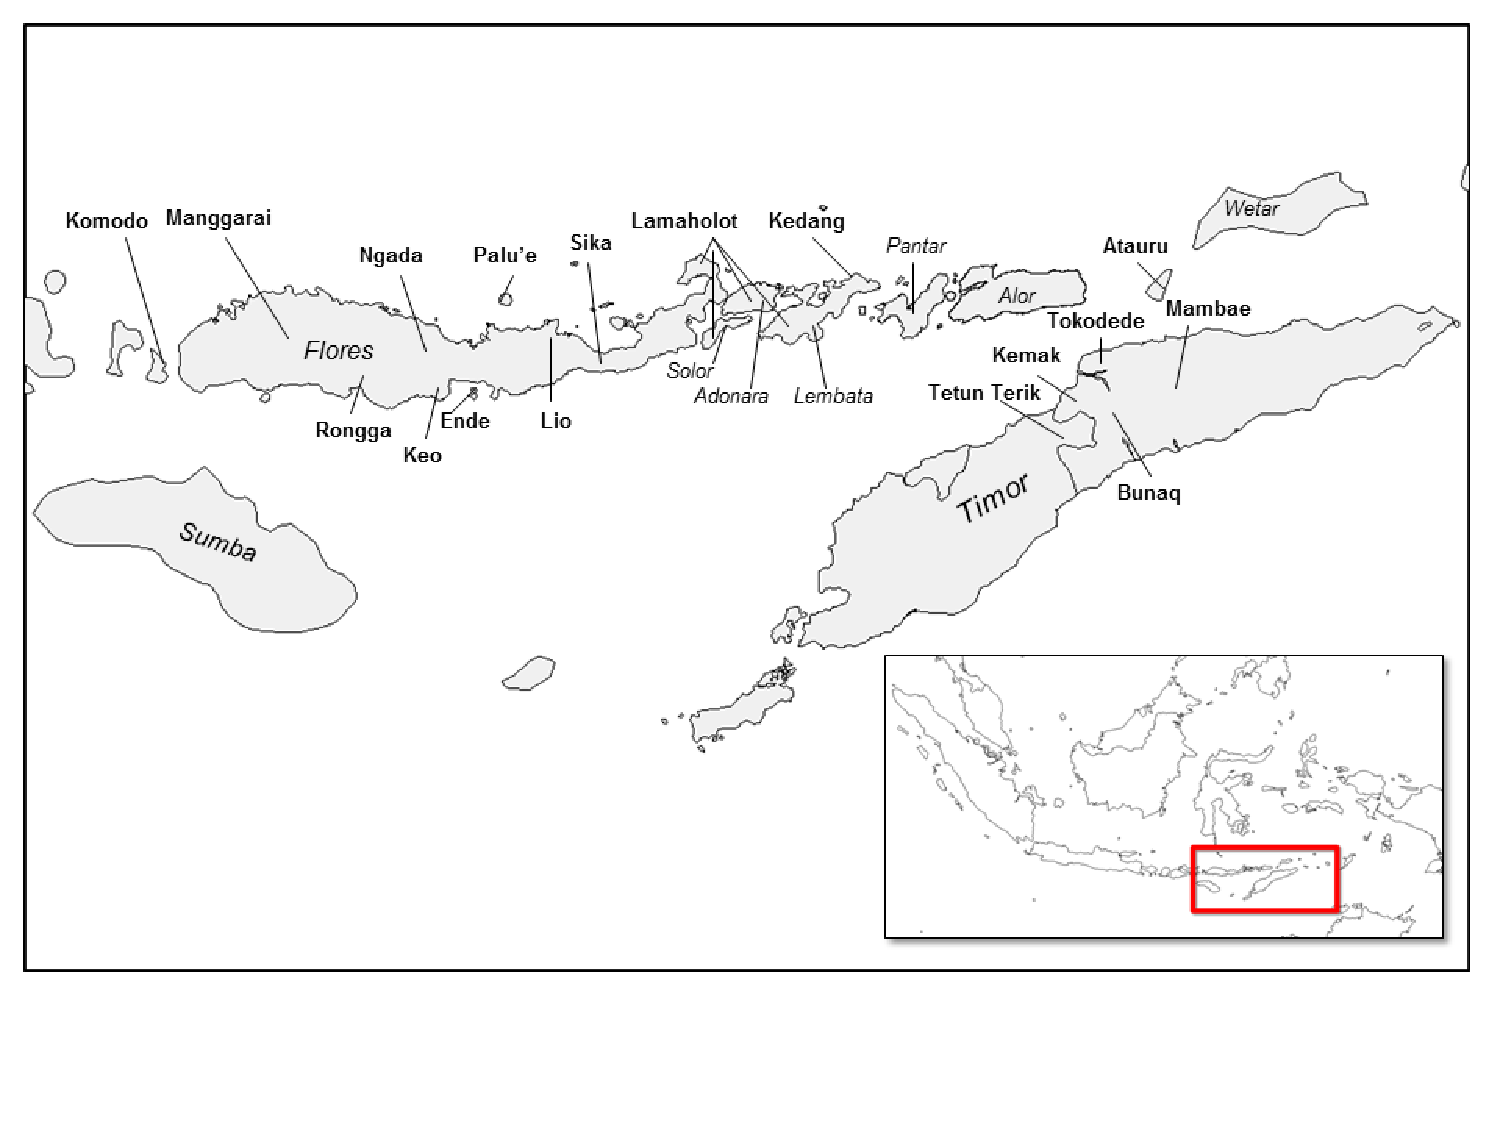
\includegraphics[width=\textwidth]{figures/ch7fig1.pdf}
% 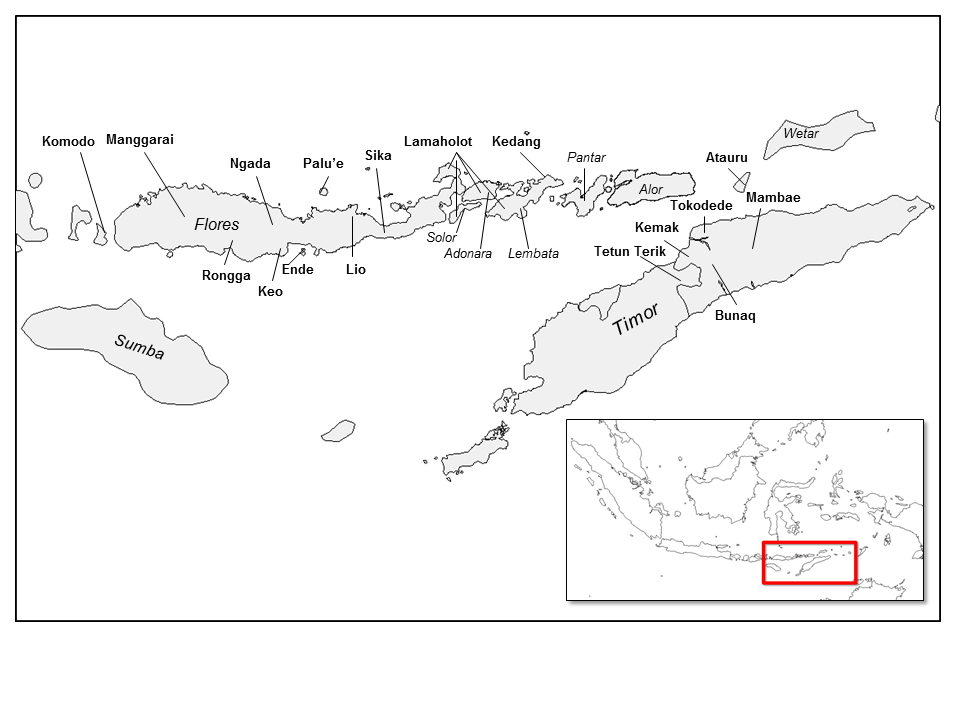
\includegraphics[width=\textwidth]{figures/ch7fig1.png}
\caption{Austronesian  languages\ilt{Austronesian language(s)} to the west and south of Alor{}-Pantar. Names in bold are language names, names in italics are names of islands.}
\label{fig:6:1}
\end{figure}

\begin{table}
 
\caption{Mixed numeral systems in proto-Austronesian\ilt{proto-Austronesian} and the Austronesian languages\ilt{Austronesian language(s)} of Flores, Lembata and Timor (1-5)}

\label{tab:6:10a}
\small 
\begin{tabularx}{\textwidth}{ll>{\it}l>{\it}l>{\it}l>{\it}l>{\it}l}
\lsptoprule
&   		  & \rm {`one'} 		& \rm  {`two'} 	& \rm  {`three'} 	& \rm  {`four'} 			& \rm  {`five'} 	\\	
\midrule 
			&  {pAN\ilt{proto-Austronesian}}&  {*esa {\Tilde}*isa} 	&  {*duSa} 	&  {*telu} 	&  {*Sepat} 			&  {*lima} 	\\
\tablevspace
{Flores} 		&  Rongga\ilt{Rongga} 	&  {\itshape  (e)sa} 			&  {\itshape  {\textturnr}ua} 	&  {\itshape  telu} 		&  {\itshape  wutu} 				&  {\itshape  lima} 		\\	
			&  Ende\ilt{Ende} 	&  {\itshape  sa} 			&  {\itshape  zua} 		&  {\itshape  tela} 		&  {\itshape  wutu} 				&  {\itshape  lima} 		\\	
			&  Ngadha\ilt{Ngadha} 	&  {\itshape  esa} 			&  {\itshape  zua} 		&  {\itshape  telu} 		&  {\itshape  vutu} 				&  {\itshape  lima} 		\\	
			&  Nage\ilt{Nage} 	&  {\itshape  esa} 			&  {\itshape  {\texthtd}ua} 	&  {\itshape  telu} 		&  {\itshape  wutu} 				&  {\itshape  lima} 		\\	
			&  Kéo\ilt{Kéo} {\dag} &  {\itshape  ha{\textglotstop}esa} 	&  {\itshape  {\textglotstop}esa rua}&  {\itshape  {\textglotstop}esa tedu}&  {\itshape  {\textglotstop}esa wutu} 	&  {\itshape  {\textglotstop}esa dima} \\	
			&  Lio\ilt{Lio} 		&  {\itshape  {\textschwa}sa} 		&  {\itshape  rua} 		&  {\itshape  t{\textschwa}lu} 	&  {\itshape  sutu} 				&  {\itshape  lima} 		\\	
\tablevspace
{Lembata} 	&  Kedang\ilt{Kedang}* 		&  {\itshape  >ude{\textglotstop}}&  {\itshape  sue} 		&  {\itshape  t{\ae}lu} 		&  {\itshape  >apa{\textglotstop}} 	&  {\itshape  leme} 		\\	
\tablevspace
{Timor} 	&  Mambae\ilt{Mambai} 		&  {\itshape  id} 			&  {\itshape  ru} 		&  {\itshape  teul} 		&  {\itshape  fat} 				&  {\itshape lim} 		\\	
		    &  Tokodede\ilt{Tokodede} 	&  {\itshape  iso} 			&  {\itshape  ru} 		&  {\itshape  telo} 		&  {\itshape  pat} 				&  {\itshape lim} 		\\	
\lspbottomrule
\end{tabularx}

\parbox{\textwidth}{
  {\dag} Kéo numerals appear with the default classifier\ist{numeral classifier} \textit{{\textglotstop}esa} and/or the prefix \textit{ha} `one'.

      * In Kedang orthography />/ preceding a vowel encodes that vowel as breathy \citep{Samely1991}.
}
\end{table}

\largerpage
It is a well-established fact that proto-Austronesian\il{proto-Austronesian} (pAN) had a decimal system, with numerals `one' through `nine' all being simple mono-morphemic words. \citet[268]{Blust2009} claims that outside of Melanesia few Austronesian languages\il{Austronesian language(s)} have innovated\is{innovation} complex - additive\is{additive numeral}, subtractive\is{subtractive numeral} or multiplicative\is{multiplicative numeral} - numerals for `one' to `ten'. The Austronesian languages\il{Austronesian language(s)} around AP, however, show a notable clustering of just such innovations\is{innovation}. We compiled numeral data for 32 Austronesian languages\il{Austronesian language(s)} spoken west and south-east of Alor and Pantar (see Appendix \ref{sec:6:app:2} and \ref{sec:6:app:3}). In these, we observe three distinct patterns of innovations\is{innovation} in the formation of numerals `six' through `nine', reflected in nine modern Austronesian languages\il{Austronesian language(s)} (\tabref{tab:6:10b}). These are: the Timor pattern (1-5, 5+1, 5+2, 5+3, 5+4, 10), the Lembata pattern (1-7, 4x2, 5+4, 10), and the Flores pattern (1-5, 5+1, 5+2, 2x4, 10-1, 10). Proto-Austronesian\il{proto-Austronesian} numerals are provided for comparative purposes in the top row. 

 
 




\begin{table}
\caption{Mixed numeral systems in proto-Austronesian\ilt{proto-Austronesian} and the Austronesian languages\ilt{Austronesian language(s)} of Flores, Lembata and Timor (6-10)\label{tab:6:13Mixed}}
\begin{tabularx}{\textwidth}{ll>{\it}l>{\it}l>{\it}l>{\it}l>{\it}l}
\lsptoprule
&   		  & \rm  {`six'} 				& \rm  {`seven'} 					& \rm  {`eight'} 						\\ 	
\midrule 		
			&  {pAN}		&  {*enem} 					&  {*pitu} 					&  {*walu} 					\\[.4em]			
{Flores} 		&  Rongga 	&    \tabtrs{2.5cm}{lima esa}{5 1} 	&  \tabtrs{2.5cm}{lima{\textturnr}ua}{ 5 2} 			&  \tabtrs{2.5cm}{\textit{{\textturnr}uambutu}}{ 2 4} 			\\[.4em]	
			&  Ende 		&    \tabtrs{2.5cm}{limasa}{5 1} 			&  \tabtrs{2.5cm}{limazua}{ 5 2} 					&  \tabtrs{2.5cm}{ruabutu}{ 2 4} 	\\[.4em]			
			&  Ngadha 	&    \tabtrs{2.5cm}{lima esa}{ 5 1} 			&  \tabtrs{2.5cm}{limarua}{ 5 2} 					&  \tabtrs{2.5cm}{ruabutu}{ 2 4} 	\\[.4em]		
			&  Nage 		&    \tabtrs{2.5cm}{lima esa}{ 5 1} 			&  \tabtrs{2.5cm}{lima zua}{ 5 2} 				&  \tabtrs{2.5cm}{zua butu}{ 2 4} 		\\[.4em]		
			&  Kéo {\dag} &    \tabtrs{2.5cm}{{\textglotstop}esa dima {\textglotstop}esa}{ 5 1}&  \tabtrs{2.5cm}{\textit{{\textglotstop}}\textit{esa dima rua}}{ 5 2} &  \tabtrs{2.5cm}{{\textglotstop}esa rua mbutu}{ 2 4} \\[.4em]		
			&  Lio 		&    \tabtrs{2.5cm}{{lima  {\textschwa}sa}}{5 1} 			&  \tabtrs{2.5cm}{lima  rua}{5 2} 					&  \tabtrs{2.5cm}{rua mbutu}{ 2 4} 			\\[.4em]		
{Lembata} 		&  Kedang* 	&    \tabtrs{2.5cm}{{>{\ae}n{\ae}ng}}{} 		&  \tabtrs{2.5cm}{pitu}{} 					&  \tabtrs{2.5cm}{butu rai}{ 4 2?} 			    	\\[.4em]		
{Timor}		 	&  Mambae 	&    \tabtrs{2.5cm}{limnai nide}{ 5 1} 			&  \tabtrs{2.5cm}{limnai rua}{ 5 2} 				&  \tabtrs{2.5cm}{limnai telu}{ 5 3} 		\\[.4em]		
			&  Tokodede 	&    \tabtrs{2.5cm}{wouniso}{ {\ob}5{\cb} 1} 			&  \tabtrs{2.5cm}{wouru}{ {\ob}5{\cb} 2} 					&  \tabtrs{2.5cm}{woutelo}{ {\ob}5{\cb} 3} 	\\[.4em]		
% \lspbottomrule
\end{tabularx}
 


\begin{tabularx}{\textwidth}{ll>{\it}l>{\it}l>{\it}l>{\it}l>{\it}l}
% \lsptoprule
			&   		  & \rm {`nine'} 	& \rm  {`ten'}\\ 
\midrule 
			&  {pAN}& {*siwa} 	&  {*puluq}\\[.4em] 
{Flores} 		&  Rongga 		&   \tabtrs{2.5cm}{taraesa}{ {\ob}10{\cb} 1 }	&  \tabtrs{2.5cm}{sambulu}{ 1 10}\\[.4em]	
			&  Ende 			&   \tabtrs{2.5cm}{trasa}{ {\ob}10{\cb} 1 }	& \tabtrs{2.5cm} {sabulu}{ 1 10}\\[.4em]
			&  Ngadha 		&   \tabtrs{2.5cm}{teresa}{ {\ob}10{\cb} 1 }	&  \tabtrs{2.5cm}{habulu}{ 1 10}\\[.4em]
			&  Nage 			&   \tabtrs{2.5cm}{tea esa}{ {\ob}10{\cb} 1 }	&  \tabtrs{2.5cm}{sa bulu}{ 1 10}\\[.4em]
			&  Kéo {\dag}		 &  \tabtrs{2.5cm} {{\textglotstop}esa tera {\textglotstop}esa}{ {\ob}1 10{\cb} 1} 	& \tabtrs{2.5cm}{hambudu}{ 1 10}\\[.4em]
			&  Lio 			&   \tabtrs{2.5cm}{t{\textschwa}ra   {\textschwa}sa}{ {\ob}10{\cb} 1 }	&  \tabtrs{2.5cm}{sambulu}{ 1 10}\\[.4em]
{Lembata} 		&  Kedang* 		&   \tabtrs{2.5cm}{leme >apa{\textglotstop}}{ 5 4} 	&  \tabtrs{2.5cm}{pulu}{1 10}\\[.4em]
{Timor} 			&  Mambae 		&   \tabtrs{2.5cm}{limnai pata}{ 5 4} 	&  \tabtrs{2.5cm}{sikul}{}\\[.4em]
			&  Tokodede 		&   \tabtrs{2.5cm}{woupat}{ {\ob}5{\cb} 4 }	&  \tabtrs{2.5cm}{sagulu}{ 1 10}\\[.4em]
\lspbottomrule
\end{tabularx}
 
\parbox{\textwidth}{
\small
  {\dag} Kéo numerals appear with the default classifier\ist{numeral classifier} \textit{{\textglotstop}esa} and/or the prefix \textit{ha} `one'.

      * In Kedang orthography />/ preceding a vowel encodes that vowel as breathy \citep{Samely1991}.
}

\label{tab:6:10b}
\end{table}

\renewcommand{\arraystretch}{1}

  
    Innovative\is{innovation} quinary numerals are found in the Austronesian languages\il{Austronesian language(s)} across the three innovative types. In the north-central Timor languages, Tokodede\il{Tokodede} and Mambae\il{Mambai}, we have quinary numerals for numerals from `six' through `nine', a pattern that stands out against the typically conservative numerals systems of the Austronesian languages\il{Austronesian language(s)} elsewhere on Timor (Naueti\il{Naueti} being an exception, see \citet{SchapperEtAl2013} on the possible reasons for the quinary numerals in Naueti). It is notable that the close inland relative of Tokodede\il{Tokodede} and Mambae\il{Mambai}, Kemak\il{Kemak}, has no base-5 numerals (see Appendix \ref{sec:6:app:3}). The appearance of this pattern in these languages may be a result of contact with speakers of AP languages spoken on the south and east coast of Alor, such as Kula\il{Kula}, Sawila\il{Sawila} and Wersing\il{Wersing}, located just a short sea crossing from the north of Timor. There is some linguistic evidence that contacts between these Alor groups and those of north-central Timor existed: the additive operators in the central-east Alor languages Sawila\il{Sawila}, Kula\il{Kula} and Wersing\il{Wersing} (see \tabref{tab:6:7}) seem to be borrowed\is{borrowing} from Tokodede\il{Tokodede} (\sectref{sec:6:6.2}). In addition, oral traditions record contacts between groups in south-east Alor and north Timor. For instance, eastern Alor groups almost invariably trace their origins to pre-historic migrations from Timor (\citealt{WellfeltEtAl2013}, Wellfelt pers. comm. 2013). Similarly, many songs in central-east Alor are sung in the Tokodede\il{Tokodede} language and mention place names such as Likusaen and Maubara, which are located in the north of Timor in the area where Tokodede is spoken \citep{WellfeltEtAl2013}. However, as \citet{WellfeltEtAl2013} argue, the directionality of the influence in the contact relations retrievable from such oral traditions and linguistic evidence is firmly flowing from Timor to Alor. The borrowing\is{borrowing} of quinary numerals from AP into Timor languages thus would appear to go against the other borrowing\is{borrowing} patterns, including that seen thus far in numerals. As such, whilst Alorese\il{Alorese} quinary numerals are the only such systems that are in contact with the Tokodede\il{Tokodede} and Mambae\il{Mambai} and seem the best candidate for the innovative\is{innovation} numeral formation, it remains to be explained why this pattern was able to spread to the Timor languages, when in oral traditions and language it is the Timor groups that are the source of influence on Alor and not a recipient of it.

The origin of the base-five numerals in the central-eastern Flores languages Rongga\il{Rongga}, Ende\il{Ende}, Ngadha\il{Ngadha}, Nage\il{Nage}, Kéo\il{Kéo}, and Lio\il{Lio} is yet more obscure. There is mounting evidence of a non-Austronesian substrate in the Austronesian languages\il{Austronesian language(s)} of the Flores region \citep[see, e.g.,][]{Capell1976,Klamer2012}. Accordingly, we may hypothesize that the quinary forms of the Flores languages reflect a prehistoric Papuan (or non-Austronesian) substrate that had a quinary system for the lower cardinals\is{cardinal numeral(s)}. However, we currently lack any evidence to link the languages forming the substrate in the central-eastern Flores region to the AP languages as we know it today -- the Flores substrate could just as well be part of a different non-Austronesian group. 

For Kedang\il{Kedang} on north Lembata, however, we are on a firmer ground to say that it formed its numeral `nine' on the basis of the quinary patterns used for `six' through `nine' in the AP languages of northern Pantar, which is located just east of the Kedang\il{Kedang} speaking area on Lembata (see Figure \ref{fig:6:1}). 
Note that the Lamaholot\il{Lamaholot} dialects spoken around Kedang\il{Kedang} in south and west Lembata all lack quinary numerals (see Appendix \ref{sec:6:app:2}) so that Kedang\il{Kedang} `nine' stands out as being different from its immediate Austronesian\il{Austronesian language(s)} neighbours. In his ethnographic study of the Kedang\il{Kedang}, \citet{Barnes1974} noted that the Kedang\il{Kedang} speakers are culturally very different from the Lamaholot\il{Lamaholot} groups on Lembata, instead showing cultural similarities with the AP groups of Alor and Pantar. For instance, unlike the Lamaholot\il{Lamaholot}, the Kedang\il{Kedang} are known for `the number of gongs [they] own and especially in the fact that [these] are used as bridewealth' \citep[15]{Barnes1974}, which is also a common practice in AP groups. The unique quinary form of Kedang\il{Kedang} `nine' may well be a trace of cultural contact between Kedang\il{Kedang} and AP speakers on Pantar, for instance in bridewealth negotiations involving gongs. 

In turn, we now investigate to what extent the numeral systems in AP languages have been influenced by nearby Austronesian languages\il{Austronesian language(s)}. In sections 4-6, we saw that some AP languages employ numerals containing morphemes that have been borrowed\is{borrowing} from Austronesian languages\il{Austronesian language(s)}, in the following five contexts: 


\begin{enumerate}
\item A reflex of pAN\ilt{proto-Austronesian} *pitu was borrowed\is{borrowing} into the Straits-West Alor languages as a base in the numeral `seven'. 

\item The Western Pantar\ilt{Western Pantar} numeral `six' \textit{hisnakkung} has an initial element \textit{his-} that is a likely Austronesian\il{Austronesian language(s)} borrowing\is{borrowing} ({\textless} PAN\ilt{proto-Austronesian} esa{\Tilde}*isa `one'), and \textit{hisnakkung} represents a partial calque of the [5 1] pattern found in Austronesian languages\il{Austronesian language(s)} of Flores. 

\item An additive\is{additive numeral} operator with the approximate form /geresin/ was borrowed\is{borrowing} into east Alor languages from Tokodede\ilt{Tokodede} (north Timor). 

\item Reflex(es) of pAN\ilt{proto-Austronesian} *Ratus `hundred' were borrowed\is{borrowing} from the Flores-Lem\-ba\-ta Austronesian languages\il{Austronesian language(s)} into the languages of Pantar, and to a lesser extent Alor.

\item Reflex(es) of pAN\ilt{proto-Austronesian} *libu `thousand' were borrowed\is{borrowing} from Flores-Lembata Austronesian languages\il{Austronesian language(s)} into AP languages across the board.  


\end{enumerate}
  The pattern for Kui\il{Kui} \textit{tadusa} `eight' seems to be formed a multiplicative\is{multiplicative numeral} pattern 2x4 due to the second element appearing to be derived from \textit{usa} `four'. This multiplicative\is{multiplicative numeral} pattern is otherwise unknown in AP languages, but is found in the Austronesian languages\il{Austronesian language(s)} of central-eastern Flores (Ende\il{Ende}, Lio\il{Lio}, Ngadha\il{Ngadha}, Rongga\il{Rongga}, Keo\il{Keo}). Whilst the Kui\il{Kui} are today not directly adjacent to any of the Austronesian languages\il{Austronesian language(s)} of Flores with multiplicative\is{multiplicative numeral} `eight', there are indications that they may have had fairly intensive contact with Austronesian\il{Austronesian language(s)} speakers from the west. Kui\il{Kui} oral tradition holds that the royal family of the group migrated to Alor from Flores (Emilie Wellfelt pers. comm.). \citet[38, fn. 36]{Hagerdal2012} cites evidence that the Kui\il{Kui} were part of a league consisting of the five princedoms Pandai, Baranusa, Blagar, Alorese and Kui. Today, Pandai, Baranusa and Alor are locations where Alorese\il{Alorese} is spoken, an Austronesian language\il{Austronesian language(s)} closely related to Lamaholot\il{Lamaholot} in the Flores region \citep{Klamer2011,Klamer2012}. In the historical period, the Kui king is also widely recorded to have owned boats running trade routes between Alor and Kupang in West Timor and islands of the Solor archipeligo (Emilie Wellfelt pers. comm., \citealt{Hagerdal2012}). It is therefore possible that the Kui were once in close contact with speakers of (an) Austronesian language(s)\il{Austronesian language(s)} from the Flores region, and that this contact might be the ultimate source of their base-4 numeral `eight'.

Finally, recall that forming `nine' by subtraction ([10]-1) is found in the Alor-Pantar languages of Straits-West-Alor, while in the Austronesian languages\il{Austronesian language(s)} of central-east Flores, monomorphemic\is{simplex numeral} `nine' (proto-Austronesian\il{proto-Austronesian} *siwa) has been replaced with a subtractive\is{subtractive numeral} compound containing two formatives: a reflex of proto-Austronesian\il{proto-Austronesian} *esa `one', and an unanalysable initial element (*tar). There is no obvious explanation how the subtractive\is{subtractive numeral} `nine' entered this group of Flores languages. Neither can we explain the origin of the subtractive\is{subtractive numeral} pattern in proto-Straits-West-Alor\il{proto-Straits-West-Alor}. We have argued that in this proto-language, subtractive\is{subtractive numeral} `nine' replaced the original pAP\il{proto-Alor-Pantar} base-five form of `nine' [5 4], and involved reflexes of pAP *nuk `one', subsequently extending the subtractive\is{subtractive numeral} system to `eight' and `seven'. So it is the subtractive\is{subtractive numeral} pattern that is similar across the Flores and Straits-West Alor groups, not the lexemes themselves. The geographical closeness of the groups, combined with the relative rarity of subtractive\is{subtractive numeral} systems in both Austronesian\il{Austronesian language(s)} and Alor-Pantar languages, may be suggestive of a (possibly ancient) structural diffusion. On the other hand, we cannot exclude the possibility that the forms were innovated independently in both groups: as \citet{SchapperEtAl2013} point out, innovation of subtractive numerals\is{subtractive numeral} has occured independently in proto-Malay\il{proto-Malay}, central Maluku and south-east Sulawesi. 

In short, contact-induced borrowings\is{borrowing} of both forms and structures (`matter' and `patterns') have played a role in shaping some of the numerals in the Alor-Pantar and nearby Austronesian languages\il{Austronesian language(s)}. Some contacts took place in historical times, and are supported by historical and ethnographic data, others are likely to be of more ancient date and must remain hypothetical. There are also similarities that cannot be traced back to contact. 

\section{Conclusions and discussion}\label{sec:6:8}
  From this comparative study of the numeral paradigms in 19 AP language varieties we draw three types of conclusions: (i) about the morphological make up of the numeral compounds; (ii) about typological rarities in the AP numeral systems, and (iii) about the subgrouping and history of the AP language group.

Morphologically, AP cardinals\is{cardinal numeral(s)} above `six' consist of minimally two formatives. Additive\is{additive numeral} base-five forms involve two (reflexes of) numerals and no marker for addition. Subtractive\is{subtractive numeral} base-ten forms involve a numeral and an unanalysable initial element that appears to go back to a morpheme originally meaning something like `less' or `take away'. With one exception, the numerals `ten' are compounds of `ten' and `one', and the decades are formed accordingly. Numerals `one hundred' and `one thousand' are structured in the same way, expressing multiplication of the base with juxtaposed numerals in which the highest numeral precedes the lowest. Numerals in between decades are expressed as phrases, involving an additive\is{additive numeral} operator (proto-AP\il{proto-Alor-Pantar} *wali({\ng}) `add, (do) again'). 

Typologically, the constellations of numerals `six' through `nine' in AP represent two rare patterns. The first rarity is the combination of a mono-morphemic `six' with quinary forms `seven' through `nine' found in many languages across the two islands, and reconsructed to proto-AP\il{proto-Alor-Pantar}. The second rarity is the occurrence of subtractive\is{subtractive numeral} base-ten systems alongside a monomorphemic\is{simplex numeral} `six' as found in the Straits-West-Alor languages. Typologically interesting are the mathematically `incorrect' numerals found in some of the languages: a `seven' that mathematically should be `four' (Straits-West Alor), a `seven' and `eight' that mathematically should be `nine' and `ten' (Western Pantar\il{Western Pantar}), and an `eight' that would literally translate as `minus four' in Kui\il{Kui}. These forms all arose through reanalysis of the numeral value of the base as different from its etymological source. Finally, it is of typological interest to consider the non-numeral lexemes that are incorporated into AP numerals: the (ad)verbs `less' and `take away' as part of subtractive numerals\is{subtractive numeral};      \textit{mi-}, an originally locative morpheme deriving decades; and the word `single' standing in for the numeral `one' in compound numerals for `six'. 

Historically, this study has provided information on the numeral system of proto-AP\il{proto-Alor-Pantar}, and additional details on affiliations and distinctions between members of the AP group that may be used as evidence to construct particular subgroups within the family. The proto-AP\il{proto-Alor-Pantar} numeral system was a mixed quinary and decimal system, with a monomorphemic\is{simplex numeral} `six' (i.e. 1, 2, 3, 4, 5, 6, [5 2], [5 3], [5 4], [10 1]). The arithmetic operations involved were addition and multiplication. Over time, the system was complicated by reorganizations of patterns as well as borrowings\is{borrowing} of numeral bases, or patterns, or both. As a result, some modern languages have introduced subtractive\is{subtractive numeral} procedures instead of, or along with, addition and multiplication. Some languages incorporated non-numeral formatives into their numerals. 

\newpage 
Numeral forms were reconstructed to different nodes in the AP family, as summarized in \tabref{tab:6:11}. The table is to be read from left to right. The left-most column represents the oldest numeral forms, that is, those that can be reconstructed to proto-AP\il{proto-Alor-Pantar}. Numerals `one' through `six' in this proto-language were monomorphemic\is{simplex numeral} forms, while `seven' through `nine' were regular quinary forms. The right-hand columns represent numeral innovations\is{innovation} which can be reconstructed to different subgroups of the AP family.\enlargethispage{1em}\footnote{The ordering of right-hand columns is by number of languages; it should not be interpreted as representing a chronology of the age of subgroups in the case of proto-Straits-West-Alor (pSWA)\il{proto-Straits-West-Alor} and proto-Pantar (pP)\il{proto-Pantar}. Naturally, proto-Central-East-Alor (pCEA)\il{proto-Central East Alor}, proto-East Alor (pEA)\il{proto-East Alor} and proto-East Alor Montane (pEAM)\il{proto-East Alor Montane} can be taken to represent a chronological sequence, since pEA\il{proto-East Alor} forms a subgroup of pCEA\il{proto-Central East Alor}, and pEAM\il{proto-East Alor Montane} a subgroup of pEA\il{proto-East Alor}.} 

\begin{sidewaystable}
\caption{Numeral (pattern) reconstructions for `one' through `ten' in AP subgroups} 

\label{tab:6:11}

\begin{tabularx}{\textwidth}{lp{2cm}p{3cm}p{2cm}p{3cm}p{2cm}p{2cm}}
\lsptoprule
& \rm Proto-Alor-Pantar\ilt{proto-Alor-Pantar} & \rm  Proto-Straits-West-Alor\ilt{proto-Straits-West-Alor} & \rm  Proto-Pantar\ilt{proto-Pantar} & \rm  Proto-Central-East-Alor\ilt{proto-Central East Alor} & \rm  Proto-East Alor\ilt{proto-East Alor} & \rm  Proto-East Alor Montane\ilt{proto-East Alor Montane}\-\\
\midrule 
`one' & *nuk &  &  &  &  & *sundana\\
`two' & *araqu &  &  &  &  & \\
`three' & *(a)tiga &  &  &  & *arasiku & \\
`four' & *buta &  &  &  &  & \\
`five' & *yiwesin &  &  &  &  & \\
`six' & *talam &  &  &  &  & \\
`seven' & \rm 5 2 & *{\texthtb}utitoga & *yewasraqo &  &  & \\
`eight' & \rm 5 3 & *turarok & *yesantig &  &  & \\
`nine' & \rm 5 4 & *tukarinuk & *yesanut &  &  & \\
`ten' & *qar &  &  & *adayaku &  & \\
\lspbottomrule
\end{tabularx}
\end{sidewaystable}

  
Translated into a tree, the reconstruction of numerals in AP languages yields the structure in Figure \ref{fig:6:2}. 


\begin{sidewaysfigure}
\caption{Tree of the AP languages based on numeral innovations\ist{innovation}}
\label{fig:6:2}

\Tree [.pAP\ilt{proto-Alor-Pantar} [.pP\ilt{proto-Pantar} [.pCP\ilt{proto-Central Pantar} [.pCEP\ilt{proto-Central Pantar} Kaera\ilt{Kaera} Sar\ilt{Sar} ] Teiwa\ilt{Teiwa} ] Deing\ilt{Deing} ] [.pSWA\ilt{proto-Straits-West-Pantar} \qroof{\parbox{1cm}{\vspace{.1cm}Blagar\ilt{Blagar}\\Reta\ilt{Retta}\\Kabola\ilt{Kabola}\\Adang\ilt{Adang}\\Hamap\ilt{Hamap}\\Klon\ilt{Klon}}}.{}  Kui\ilt{Kui}\raisebox{.4cm}[-2cm]{\hspace{-.2cm}?} West{ }Pantar\ilt{Western Pantar}\raisebox{.4cm}[-2cm]{\hspace{-1.1cm}?\hspace{1cm}} ]!\qsetw{4.3cm} \parbox{.1cm}{Abui\ilt{Abui}} [.pCEA\ilt{proto-Central East Alor} Kamang\ilt{Kamang} [.pEA\ilt{proto-East Alor} Wersing\ilt{Wersing} [.pEAM\ilt{proto-East Alor Montane} Sawila\ilt{Sawila} Kula\ilt{Kula} ]  ]  ]  ] 

%\includegraphics[width=4.1874in,height=2.3957in,width=\textwidth]{a5c369bcf9e04c7abcbe33fc0d1515af-img1}
\end{sidewaysfigure}

We see that that there are patterns and forms found in the Pantar languages (except Western Pantar\il{Western Pantar}) are clearly separate from those in the languages of Alor; the Straits West Alor languages (Blagar\il{Blagar}, Reta\il{Retta}, Kabola\il{Kabola}, Adang\il{Adang}, Hamap\il{Hamap}, Klon\il{Klon}) share patterns and forms amongst themselves that are not shared with other AP languages; and we argued the same to be the case for the languages of central and east Alor. The subgrouping membership of the Kui\il{Kui} and Western Pantar\il{Western Pantar} is problematic; their grouping within pSWA\il{proto-Straits-West-Alor} is tentative and rests on their possessing some innovative\is{innovation} morphemes (i.e., reflexes of *{\texthtb}uti- and *tukari) in common with the main Straits-West Alor languages proper, though with different functions in Kui\il{Kui} and Western Pantar\il{Western Pantar}.

The preliminary reconstruction of Proto-AP\il{proto-Alor-Pantar} based on sound changes\is{sound change} as reported in \citet{HoltonEtAl2012} and \citep{HoltonRobinsonTVhistory} focuses on showing the relatedness of all AP languages. Little work has been done on the sound changes\is{sound change} defining lower-level subgroups of AP languages. Nevertheless, there are some correspondences that can be observed. For instance, the pSWA\il{proto-Straits-West-Alor} subgroup we define (without the problematic inclusion of Kui\il{Kui} and Western Pantar\il{Western Pantar}) is also supported by the sound change\is{sound change} *s > h. Further study of lower level sound changes\is{sound change} is needed to test whether all the subgroups we posit here on the basis of the morphological evidence of numerals are valid. 

In sum, cardinal numerals\is{cardinal numeral(s)} in the Alor-Pantar languages are fertile ground for understanding how diverse numeral systems can evolve in related languages. In particular, Alor-Pantar languages provide us with unique, typological insights into the historical changes and influences that can complicate and prompt reorganizations of patterns of numeral formation and borrowings\is{borrowing} into the numeral paradigm.
 
 \newpage 
\section{Sources} \label{sec:6:9}
Sources of the language data cited in the text and the Appendices are given in the table below. We provide information about the dialect in cases where unpublished sources are used, or where multiple dialects are cited. \vspace{.2cm}



\begin{tabularx}{\textwidth}{p{5cm}p{6cm}} 
Abui\ilt{Abui} (AP) 	&  \citet{Kratochvil2007},\par Schapper fieldnotes 2010 	  \\
Adang\ilt{Adang} (AP, Pitungbang dialect) 	&  Robinson fieldnotes 2010 	 \\
Alorese\ilt{Alorese} (AN\ilt{Austronesian language(s)}) 	&  \citet{Klamer2011} 	  \\
Amarasi\ilt{Amarasi} (AN) 	&  \citet{BaniEtAl2011} 	 \\
Atauro\ilt{Atauro} (AN) 	&  Schapper fieldnotes 2007 	  \\
Blagar\ilt{Blagar} (AP, Bama dialect) 	&  Robinson fieldnotes 2010 	 \\
Blagar (AP, Dolabang dialect) 	&  Hein Steinhauer p.c. 2011 	 \\
Bunaq\ilt{Bunaq} (TAP, Lamaknen) 	&  \citet{Schapper2009} 	\\
Bunaq (TAP, Manufahi) 	&  Schapper fieldnotes 2007 	 \\
Dadu'a\ilt{Dadu'a} (a.k.a. Galoli) (AN) 	&  \citet{Penn2006} 	  \\
Dhao\ilt{Dhao} 	&  \citet{GrimesEtAl2008} 	 \\
Deing\ilt{Deing} (AP) 	&  B. Volk fieldnotes 2008 	 \\
Ende\ilt{Ende} (AN) 	&    \citet{AokiEtAl1993} 	  \\
Hamap\ilt{Hamap} (AP) 	&  Baird fieldnotes 2003 	  \\
Idate\ilt{Idate} (AN) 	&  Klamer fieldnotes  2002 	  \\
Ilongot\ilt{Ilongot} (AN) 	&  ABVD	  \\
Kabola\ilt{Kabola} (AP) 	&  Robinson fieldnotes 2010 	  \\
Kaera\ilt{Kaera} (AP) 	&  Klamer fieldnotes 2005 	  \\
Kamang\ilt{Kamang} (AP) 	&  Schapper fieldnotes 2010, 2011 	 \\
Kedang\ilt{Kedang} (AN) 	&  \citet{Samely1991} 	 \\
Kemak\ilt{Kemak} (AN, Atabai dialect) 	&  Klamer fieldnotes 2002 	\\
Kéo\ilt{Kéo} (AN) 	&  \citet{Baird2002} 	 \\
Klon\ilt{Klon} (AP) 	&  \citet{Baird2008} 	\\
Komodo\ilt{Komodo} (AN) 	&  \citet{Verheijen1982} 	\\
Kui\ilt{Kui} (AP) 	&  Baird fieldnotes 2003, Holton\par fieldnotes 2010 	\\
Kula\ilt{Kula} (AP) 	&  Holton fieldnotes 2010,\par Nicholas Williams p.c. 2011 	  \\
Lakalei\ilt{Lakalei} (AN\ilt{Austronesian language(s)}) 	&  Klamer fieldnotes  2002\\
\end{tabularx}

\begin{tabularx}{\textwidth}{p{5cm}p{6cm}}
Lamaholot\ilt{Lamaholot}\par (AN, Lewoingu dialect) 	&   \citet{NishiyamaEtAl2007}\\
Lamaholot\par (AN, Lewotobi dialect) 	&  Naonori Nagaya p.c. 2011\\
Lamaholot\par (AN, Lewolema dialect) 	&  \citet{Pampus2001}\\
Lamaholot\par (AN, Solor dialect) 	&  Klamer fieldnotes  2002\\
Lamaholot\par (AN, Adonara) 	&  Philippe Grangé p.c. 2011\\
Lamaholot\par (AN, Lamalera dialect) 	&  \citet{Keraf1978}\\
Lio\ilt{Lio} (AN) 	&  \citet[127-137, 44, 57, 60, 75, 110]{SawardoEtAl1987}, \citet{Arndt1933}\\
Mambae\ilt{Mambai} (AN, Ainaro dialect) 	&  Schapper fieldnotes 2007\\
Manggarai\ilt{Manggarai} (AN) 	&  \citet[518]{Verheijen1967};\par \citet[173]{Verheijen1970}\\
Nage\ilt{Nage} (AN) 	&  Gregory Forth p.c. 2011\\
Ngadha\ilt{Ngadha} (AN) 	&  \citet{Arndt1961}\\
Palu'e\ilt{Palu'e} (AN) 	&  ABVD \\
Reta\ilt{Retta} (AP) 	&  Robinson fieldnotes 2010\\
Rembong\ilt{Rembong} (AN) 	&  \citet{Verheijen1978}\\
Rongga\ilt{Rongga} (AN) 	&  \citet{ArkaEtAl2007}\\
Sar\ilt{Sar} (AP) 	&  Baird fieldnotes 2003;\par Robinson fieldnotes 2010\\
Sika\ilt{Sika} (AN) 	&  \citet{PareiraEtAl1998,Calon1890}\\
Teiwa\ilt{Teiwa} (AP) 	&  \citet{Klamer2010grammar}\\
Tetun Fehan\ilt{Tetun Fehan} (AN) 	&  \citet[100]{VanKlinken1999}\\
Tokodede\ilt{Tokodede} (AN, Licissa dialect) 	&  Schapper fieldnotes 2007\\
Uab Meto\ilt{Uab Meto} (AN) 	&  \citet[421-424]{Middelkoop1950}\\
Ujir (AN) & Schapper fieldnotes\\
Waima'a\ilt{Waima'a} (AN) 	&  \citet{Hull2002}\\
Western Pantar\ilt{Western Pantar} (AP) 	&  \citet{Holtonnda} \\
Wersing\ilt{Wersing} (AP) 	&  Holton fieldnotes 2010,\par \citet{SchapperEtAltawersing}\\
\end{tabularx}

\clearpage
\newpage
\startappendix
\subsection{Cardinal numerals\ist{cardinal numeral(s)} in the Alor-Pantar languages}\label{sec:6:app:1}
Varieties within a language are indicated by the name of one of the places where the dialect is spoken, though often dialects cover more than one place.


\begin{table}[h!]
\caption{Numerals `one' through `four'}
\label{tab:6:12}
\begin{tabularx}{\textwidth}{lXllll}
\lsptoprule
{Location} & {Language} & {`one'} & {`two'} & {`three'} & {`four'}\\
\midrule 
{Pantar} & {Western Pantar\ilt{Western Pantar}} & {\itshape anuku} & {\itshape alaku} & {\itshape atiga} & {\itshape atu} \\
 & {Deing\ilt{Deing}} & {\itshape nuk} & {\itshape raq} & {\itshape atig} & {\itshape ut}\\
 & {Sar\ilt{Sar}} & {\itshape nuk} & {\itshape raq} & {\itshape tig} & {\itshape ut}\\
 & {Teiwa\ilt{Teiwa}} & {\itshape nuk} & {\itshape (ha)raq} & {\itshape jerig} & {\itshape ut}\\
 & {Kaera\ilt{Kaera}} & {\itshape nuk(u)} & {\itshape (a)rax-} & {\itshape (i/u)tug} & {\itshape ut}\\
{ Straits} & {Blagar-Bama\ilt{Blagar}} & {\itshape nuku} & {\itshape akur} & {\itshape tuge} & {\itshape ut}\\
 & {Blagar-Dolabang} & {\itshape nu} & {\itshape aru} & {\itshape tue} & \textit{{\texthtb}}\textit{uta}\\
 & {Reta\ilt{Retta}} & {\itshape anu} & {\itshape alo} & {\itshape atoga} & \textit{w/{\texthtb}}\textit{uta}\\
{ W Alor} & {Kabola\ilt{Kabola}} & {\itshape nu} & {\itshape olo} & {\itshape towo} & {\itshape ut}\\
 & {Adang\ilt{Adang}} & {\itshape nu} & {\itshape alo} & {\itshape tuo} & {\itshape ut}\\
 & {Hamap\ilt{Hamap}} & {\itshape nu} & {\itshape alo} & {\itshape tof} & {\itshape ut}\\
 & {Klon\ilt{Klon}} & {\itshape nuk} & {\itshape orok} & {\itshape to{\ng}} & {\itshape ut}\\
 & {Kui\ilt{Kui}} & {\itshape nuku} & {\itshape oruku} & {\itshape siwa} & {\itshape usa}\\
{ C\&E Alor} & {Abui\ilt{Abui}} & {\itshape nuku} & {\itshape ajoku} & {\itshape sua} & {\itshape buti}\\
 & {Kamang\ilt{Kamang} (Atoitaa)} & {\itshape nok} & {\itshape ok} & {\itshape su} & {\itshape biat}\\
 & {Kamang (Takailubui)} & {\itshape nok} & {\itshape ok} & {\itshape su} & {\itshape biat}\\
 & {Sawila\ilt{Sawila}} & {\itshape sundana} & {\itshape jaku} & {\itshape tuo} & {\itshape araːsiːku}\\
 & {Kula\ilt{Kula}} & {\itshape sona} & {\itshape jakwu} & {\itshape tu} & {\itshape arasiku}\\
 & {Wersing\ilt{Wersing}} & {\itshape no} & {\itshape joku} & {\itshape tu} & {\itshape arasoku}\\
\lspbottomrule
\end{tabularx}
\end{table}

 

\begin{sidewaystable}
\caption{Numerals `five' through `nine'} 
\label{tab:6:13}

\begin{tabularx}{\textwidth}{Xllllll}
\lsptoprule

{Location} & {Language} & {`five'} & {`six'} & {`seven'} & {`eight'} & {`nine'}\\
\midrule 
{ Pantar} & {Western Pantar\ilt{Western Pantar}} & {\itshape jasi{\ng}} & {\itshape hisnakku{\ng}} & {\itshape betalaku} & {\itshape betiga} & {\itshape anukutanna{\ng}}\\
 & {Deing\ilt{Deing}} & {\itshape asan} & {\itshape tala{\ng}} & {\itshape jewasrak} & {\itshape santig} & {\itshape sanut}\\
 & {Sar\ilt{Sar}} & {\itshape jawan} & {\itshape teja{\ng}} & {\itshape jisraq} & {\itshape jinatig} & {\itshape jinaut}\\
 & {Teiwa\ilt{Teiwa}} & {\itshape jusan} & {\itshape tiaːm} & {\itshape jesraq} & {\itshape jesnerig} & \textit{jesna}\textit{{\textglotstop}}\textit{ut}\\
 & {Kaera\ilt{Kaera}} & {\itshape isim} & {\itshape tiaːm} & {\itshape jesrax-} & {\itshape jentug} & {\itshape jeniut}\\
{ Straits} & {Blagar-Bama\ilt{Blagar}} & {\itshape isi{\ng}} & {\itshape taja{\ng}} & {\itshape titu} & {\itshape tuakur} & {\itshape tukurunuku}\\
 & {Blagar-Dolabang} & {\itshape isi{\ng}} & {\itshape tali{\ng}} & \textit{{\texthtb}}\textit{ititu} & {\itshape tuaru} & {\itshape turinu}\\
 & {Reta\ilt{Retta}} & {\itshape aveha{\ng}} & {\itshape talaun} & {\itshape bititoga} & {\itshape tulalo} & {\itshape tukanu}\\
{ W Alor} & {Kabola\ilt{Kabola}} & {\itshape iwese{\ng}} & {\itshape tala{\ng}} & {\itshape wutito} & {\itshape turlo} & \textit{ti}\textit{{\textglotstop}}\textit{inu}\\
 & {Adang\ilt{Adang}} & {\itshape ifihi{\ng}} & {\itshape tala{\ng}} & \textit{itit}\textit{{\textopeno}} & {\itshape turlo} & \textit{ti}\textit{{\textglotstop}}\textit{enu}\\
 & {Hamap\ilt{Hamap}} & {\itshape ivehi{\ng}} & {\itshape tala{\ng}} & {\itshape itito} & {\itshape turalo} & {\itshape tieu}\\
 & {Klon\ilt{Klon}} & {\itshape eweh} & {\itshape tlan} & {\itshape uso{\ng}} & {\itshape tidorok} & {\itshape tukainuk}\\
 & {Kui\ilt{Kui}} & {\itshape jesan} & {\itshape talama} & {\itshape jesaroku} & {\itshape tadusa} & {\itshape jesanusa}\\
{ C \& E Alor} & {Abui\ilt{Abui}} & {\itshape jeti{\ng}} & {\itshape talaːma} & {\itshape jeti{\ng}ajoku} & {\itshape jeti{\ng}sua} & {\itshape jeti{\ng}buti}\\
 & {Kamang\ilt{Kamang} (Takailubui)} & {\itshape wesi{\ng}} & \textit{taːma} & {\itshape wesi{\ng}ok} & {\itshape wesi{\ng}su} & {\itshape wesi{\ng}biat}\\
 & {Kamang (Atoitaa)} & {\itshape iwesi{\ng}} & \textit{isi{\ng}nok} & {\itshape isi{\ng}ok} & {\itshape isi{\ng}su} & {\itshape isi{\ng}biat}\\
 & {Sawila\ilt{Sawila}} & {\itshape joːti{\ng}} & {\itshape joːti{\ng}sundana} & {\itshape joːti{\ng}jaku} & {\itshape joːti{\ng}tuo} & {\itshape joːti{\ng}araːsiːku}\\
 & {Kula\ilt{Kula}} & {\itshape jawatena} & {\itshape jawatensona} & {\itshape jawatenjakwu} & {\itshape jawatentu} & {\itshape jawatenarasiku}\\
 & {Wersing\ilt{Wersing}} & {\itshape weti{\ng}} & {\itshape weti{\ng}nu{\ng}} & {\itshape weti{\ng}joku} & {\itshape weti{\ng}tu} & {\itshape weti{\ng}arasoku}\\
\lspbottomrule
\end{tabularx}
\end{sidewaystable}


\begin{table}
\caption{Numerals `ten' and the formation of decades}
\label{tab:6:14}

\begin{tabularx}{\textwidth}{Xllll}
\lsptoprule
 &  & {`ten'} & {`twenty'} & {`thirty'}\\
\midrule 
{Pantar} & {Western Pantar\ilt{Western Pantar}} & {\itshape ke anuku} & {\itshape ke alaku} & {\itshape ke atiga}\\
 & {Deing\ilt{Deing}} & {\itshape qar nuk} & {\itshape qar raq} & {\itshape qar atig}\\
 & {Sar\ilt{Sar}} & {\itshape qar nuk} & {\itshape qar raq} & {\itshape qar tig}\\
 & {Teiwa\ilt{Teiwa}} & {\itshape qaːr nuk} & {\itshape qaːr raq} & {\itshape qaːr jerig}\\
 & {Kaera\ilt{Kaera}} & {\itshape xar nuko} & {\itshape xar raxo} & {\itshape xar tug}\\
{Straits} & {Blagar-Bama\ilt{Blagar}} & {\itshape qar nuku} & \textit{qar} \textit{akur} & \textit{qar} \textit{tuge}\\
 & {Blagar-Dolabang} & \textit{{\textglotstop}}\textit{ari nu} & \textit{{\textglotstop}}\textit{ari} \textit{aru} & \textit{{\textglotstop}}\textit{ari} \textit{tue}\\
 & {Reta\ilt{Retta}} & {\itshape kara nu} & \textit{kara} \textit{alo} & \textit{kara} \textit{atoga}\\
{West Alor} & {Kabola\ilt{Kabola}} & {\itshape kar nu} & \textit{kar} \textit{ho(}\textit{{\textglotstop}}\textit{)olo} & \textit{kar} \textit{towo}\\
 & {Adang\ilt{Adang}} & \textit{{\textglotstop}}\textit{er nu} & \textit{{\textglotstop}}\textit{er} \textit{alo} & \textit{{\textglotstop}}\textit{er} \textit{tuo}\\
 & {Hamap\ilt{Hamap}} & {\itshape air nu} & \textit{air} \textit{alo} & \textit{air} \textit{tof}\\
 & {Klon\ilt{Klon}} & {\itshape kar  nuk} & \textit{kar} \textit{orok} & \textit{kar} \textit{to}\textit{{\ng}}\\
 & {Kui\ilt{Kui}} & {\itshape kar nuku} & \textit{kar} \textit{oruku} & \textit{kar} \textit{siwa}\\
{C \& E Alor} & {Abui\ilt{Abui}} & {\itshape kar nuku}  & \textit{kar} \textit{ajoku} & \textit{kar} \textit{sua}\\
 & {Kamang\ilt{Kamang}} & {\itshape ataːk nok} & {\itshape ataːk ok} & {\itshape ataːk su}\\
 & {Sawila\ilt{Sawila}} & {\itshape adaːku} & \textit{adaːku} \textit{maraku} & {\itshape adaːku matua}\\
 & {Kula\ilt{Kula}} & {\itshape adajakwu} & {\itshape mijakwu} & {\itshape mitua}\\
 & {Wersing\ilt{Wersing}} & {\itshape adajoku} & {\itshape adajoku mijoku} & {\itshape adajoku mitu}\\
\lspbottomrule
\end{tabularx}
\end{table}
 

\begin{sidewaystable}

\caption{Numerals with bases `100' and `1000'}
\label{tab:6:15}

\begin{tabularx}{\textwidth}{XXXXXX}
\lsptoprule
 &  & {`100'} & {`200'} & {`1000'} & {`2000'}\\
\midrule 
{Pantar} & West Pantar\ilt{Wersing} & {\itshape ratu} & {\itshape ratu alaku} & {\itshape (a)ribu (ye)} & {\itshape ribu (alaku)}\\
 & Deing\ilt{Deing} & {\itshape aratu nuk} & {\itshape aratu raq} & {\itshape aribu nuk} & {\itshape aribu raq}\\
 & Sar\ilt{Sar} & {\itshape ratu nuk} & {\itshape ratu raq} & {\itshape ribu nuk} & {\itshape ribu raq}\\
 & Teiwa\ilt{Teiwa} & {\itshape ratu nuk} & {\itshape ratu (ha)raq} & {\itshape ribu nuk} & {\itshape ribu (ha)raq}\\
 & Kaera\ilt{Kaera} & {\itshape ratu nuk} & {\itshape ratu rax-} & {\itshape ribu nuk} & {\itshape ribu rax-}\\
{Straits} & Blagar-Bama\ilt{Blagar} & {\itshape ratu nuku} & {\itshape ratu akur} & {\itshape ribu nuku} & {\itshape ribu akur}\\
 & Blagar-Dolabang & {\itshape ratu nu} & {\itshape ratu aru} & {\itshape ribu nu} & {\itshape ribu aru}\\
 & Reta\ilt{Retta} & {\itshape ratu anu} & {\itshape ratu alo} & {\itshape ribu ano} & {\itshape ribu alo}\\
{W Alor} & Kabola\ilt{Kabola} & {\itshape rat nu} & \textit{rat} \textit{ho(}\textit{{\textglotstop}}\textit{)olo} & {\itshape rib nu} & \textit{rib} \textit{ho(}\textit{{\textglotstop}}\textit{)olo}\\
 & Adang\ilt{Adang} & {\itshape rat nu} & {\itshape rat alo} & {\itshape rib nu} & {\itshape rib alo}\\
 & Hamap\ilt{Hamap} & {\itshape rat nu} & {\itshape rat alo} & \textit{{}---}{\dag} & {\itshape {}---}\\
 & Klon\ilt{Klon} & {\itshape eska nok} & {\itshape eska orok} & {\itshape {}---} & {\itshape {}---}\\
 & Kui\ilt{Kui} & {\itshape asaga} & {\itshape asaga oruku} & {\itshape rab nuku} & {\itshape rab oruku}\\
{C \& E Alor} & Abui & {\itshape aisaha nu} & {\itshape aisaha ajoku} & {\itshape rifi nuku} & {\itshape rifi ajoku}\\
 & Kamang\ilt{Kamang} (A/T) & {\itshape asaka nok} & {\itshape asaka ok} & {\itshape libu nok} & {\itshape libu ok}\\
 & Sawila\ilt{Sawila} & {\itshape asaka dana} & {\itshape asaka jaku} & {\itshape riːbu dana} & {\itshape riːbu jaku}\\
 & Kula\ilt{Kula} & {\itshape gasaka} & {\itshape gasaka jakwana} & {\itshape rib dena} & {\itshape {}---}\\
 & Wersing\ilt{Wersing} & {\itshape aska} & {\itshape aska joku} & {\itshape ribu no} & {\itshape {}---}\\
\lspbottomrule
\end{tabularx}
 
{\dag} `\textit{{}---}' denotes that no data is available for this numeral
 
\end{sidewaystable}
 
 
 
\subsection{Numerals `one' to `ten' in Austronesian languages\ilt{Austronesian language(s)} W of Alor-Pantar}\label{sec:6:app:2} 

\renewcommand{\arraystretch}{1.2}
\begin{table}[H]
\small
\caption{Numerals `one' to `five' in Austronesian languages W of Alor-Pantar.}  
\begin{tabularx}{\textwidth}{XXlllll}
\lsptoprule
{Location} & {Language} & {`one'} & {`two'} & {`three'} & {`four'} & {`five'} \\
\midrule 
			& { PAN\ilt{proto-Austronesian}}		& {*esa{\Tilde}*isa} & {*duSa} & {*telu} & {*Sepat} & {*lima} \\
{Komodo}			& {Komodo\ilt{Komodo}} 			& {\itshape sa, se-} & {\itshape rua} & {\itshape telu} & {\itshape pa{\textglotstop}} & {\itshape lima} \\
{Flores} 		& {Manggarai\ilt{Manggarai}} 		& {\itshape esa} & {\itshape sua} & {\itshape telu} & {\itshape pat} & {\itshape lima} \\
			& {Rongga\ilt{Rongga}} 			& {\itshape (e)sa} & \textit{{\textturnr}}\textit{ua} & {\itshape telu} & {\itshape wutu} & {\itshape lima} \\
			& { Rembong\ilt{Rembong}} 		& {\itshape sa, sa{\textglotstop}} & {\itshape zta} & {\itshape telu} & {\itshape pat} & {\itshape lima} \\
			& { Ende\ilt{Ende}} 			& {\itshape sa} & {\itshape zua} & {\itshape tela} & {\itshape wutu} & {\itshape lima} \\
			& { Ngadha\ilt{Ngadha}} 			& {\itshape esa} & {\itshape zua} & {\itshape telu} & {\itshape vutu} & {\itshape lima} \\
			& {Nage\ilt{Nage}} 			& {\itshape esa} & {\itshape {\texthtd}ua} & {\itshape telu} & {\itshape wutu} & {\itshape lima} \\
			& {Kéo\ilt{Kéo}}{\dag} 		& {\itshape ha{\textglotstop}esa} & {\itshape {\textglotstop}esa rua} & {\itshape {\textglotstop}esa tedu} & {\itshape {\textglotstop}esa wutu} & {\itshape {\textglotstop}esa dima} \\
			& { Lio\ilt{Lio}} 			& {\itshape {\textschwa}sa} & {\itshape rua} & {\itshape t{\textschwa}lu} & {\itshape sutu} & {\itshape lima} \\
			& { Sika\ilt{Sika}} 			& {\itshape ha} & {\itshape rua} & {\itshape t{\textepsilon}lu} & {\itshape hutu} & {\itshape lima} \\
			& { Palu'e\ilt{Palu'e}} 			& {\itshape a} & {\itshape rua} & {\itshape t{\textschwa}lu} & \textit{{\texthtb}}\textit{a} & {\itshape lima} \\
			& { Lamaholot-Lewoingu\ilt{Lamaholot}} 	& {\itshape to{\textglotstop}u} & {\itshape rua} & {\itshape t{\textschwa}lo} & {\itshape pak} & {\itshape lema} \\
			& { Lamaholot-Lewotobi} 			& {\itshape to{\textglotstop}u} & {\itshape rua} & {\itshape t{\textschwa}lo~} & {\itshape pa} & {\itshape lema~} \\
			& { Lamaholot-Lewolema} 			& {\itshape to{\textglotstop}u} & {\itshape rua} & \textit{t}\textit{{\textschwa}lo} & {\itshape pat} & {\itshape lema} \\
{Solor}			& { Lamaholot-} {Solor} 			& {\itshape to{\textglotstop}u} & {\itshape rua} & \textit{t}\textit{{\textschwa}lo} & {\itshape pa} & {\itshape lema} \\
{Adonara} 		& { Lamaholot-} {Adonara} 		& {\itshape to{\textglotstop}u} & {\itshape rua} & \textit{t}\textit{{\textschwa}lo} & {\itshape pat} & {\itshape lema} \\
{Lembata (Lomblen)}  	& {Lamaholot-Lamalera}			& {\itshape tou} & {\itshape rua} & {\itshape telo} & {\itshape pa} & {\itshape lema} \\
		        & {Kedang\ilt{Kedang}}{\dag} 	& {\itshape >ude{\textglotstop}} & {\itshape sue} & {\itshape t{\ae}lu} & \textit{>apa}\textit{{\textglotstop}} & {\itshape leme} \\
		        & { Alorese\ilt{Alorese}-} {Baranusa} 	& {\itshape to} & {\itshape rua} & {\itshape talau} & {\itshape pa} & {\itshape lema} \\
{Pantar}  	    	& {Alorese-} {Alor Kecil} 		& {\itshape tou}& {\itshape rua} & {\itshape telo} & {\itshape pa} & {\itshape lema} \\
\lspbottomrule
\end{tabularx} 
\parbox{\textwidth}{
{\dag} Kéo\ilt{Kéo} numerals appear with the default classifier\is{numeral classifier} \textit{{\textglotstop}}\textit{esa} and/or the prefix \textit{ha} `one'.  In Kedang\ilt{Kedang} orthography />/ preceding a vowel encodes that vowel as breathy \citep{Samely1991}
}

\end{table}


\begin{table}[H]
\caption{Numerals `six' to `ten' in Austronesian languages W of Alor-Pantar}
\scriptsize 
\begin{tabularx}{\textwidth}{p{1.1cm}p{1.1cm}llllX}
\lsptoprule
{Location} & {Language} & 		  {`six'} & {`seven'} & {`eight'} & {`nine'} & {`ten'}\\
\midrule
			& { PAN\ilt{proto-Austronesian}}	&	 {*enem} & {*pitu} & {*walu} & {*siwa} & {*puluq}\\
{Komodo}			& {Komodo\ilt{Komodo}} 		&	 {\itshape nemu} & {\itshape pitu} & {\itshape walu} & {\itshape siwa} & {\itshape pulu, sampulu}\\
{Flores} 		& {Manggarai\ilt{Manggarai}} 	&		 {\itshape enem} & {\itshape pitu} & {\itshape alo} & {\itshape ciok} & {\itshape pulu\par cempulu\par  cepulu\par  campulu}\\
			& {Rongga\ilt{Rongga}} 		&		 {\itshape limaesa} & \textit{lima}\textit{{\textturnr}}\textit{ua} & \textit{{\textturnr}}\textit{uambutu} & {\itshape taraesa} & {\itshape sambulu}\\
			& { Rembong\ilt{Rembong}} 	&		 {\itshape non} & {\itshape pitu{\textglotstop}} & {\itshape walu{\textglotstop}} & {\itshape siwa{\textglotstop}} & {\itshape (se)puluh / pulu{\textglotstop}}\\
			& { Ende\ilt{Ende}} 		&		 {\itshape limasa} & {\itshape limazua} & {\itshape ruabutu} & {\itshape trasa} & {\itshape sabulu}\\
			& { Ngadha\ilt{Ngadha}} 		&	 {\itshape limaesa} & {\itshape limarua} & {\itshape ruabutu} & {\itshape teresa} & {\itshape habulu}\\
			& {Nage\ilt{Nage}} 		&		 {\itshape lima esa} & {\itshape lima zua} & {\itshape zua butu} & {\itshape tea esa} & {\itshape sa bulu}\\
			& {Kéo\ilt{Kéo}}{\dag} 	&		 {\itshape {\textglotstop}esa dima {\textglotstop}esa} & {\itshape {\textglotstop}esa} {\itshape dima rua} & {\itshape {\textglotstop}esa} {\itshape rua mbutu} & {\itshape {\textglotstop}esa} {\itshape tera {\textglotstop}esa} & {\itshape ha~mbudu}\\
			& { Lio\ilt{Lio}} 		&		 {\itshape lima  {\textschwa}sa} & {\itshape lima rua} & {\itshape rua mbutu} & {\itshape t{\textschwa}ra  {\textschwa}sa} & {\itshape sambulu}\\
			& { Sika\ilt{Sika}} 		&		 {\itshape {\textepsilon}na} & {\itshape pitu} & {\itshape walu} & {\itshape hiwa} & {\itshape pulu\par pulu ha}\\
			& { Palu'e\ilt{Palu'e}} 		&	 {\itshape {\textschwa}ne} & \textit{{\texthtb}}\textit{itu} & {\itshape valu} & {\itshape iva} & {\itshape apulu}\\
			& { Lamaholot-Lewoingu\ilt{Lamaholot}}& 		 {\itshape n{\textschwa}m{\textschwa}n} & {\itshape pito} & {\itshape buto} & {\itshape hiwa} & {\itshape pulo}\\
			& { Lamaholot-Lewotobi} 		&	 {\itshape namu} & {\itshape pito~} & {\itshape buto} & {\itshape hiwa} & {\itshape pulo}\\
			& { Lamaholot-Lewolema} 		&	 {\itshape n{\textschwa}m({\textschwa})} & {\itshape pito} & {\itshape buto} & {\itshape hiwa} & {\itshape pulok}\\
{Solor}			& { Lamaholot-} {Solor} 		&	 \textit{n}\textit{{\textschwa}}\textit{m}\textit{\~{u}} & {\itshape pito} & {\itshape wutu} & {\itshape hiwa} & {\itshape pulo{\textglotstop}

  pulok}\\
{Adonara} 		& { Lamaholot-} {Adonara} 	&		 \textit{n}\textit{{\textschwa}}\textit{m(}\textit{{\textschwa}}\textit{)} & {\itshape pito} & {\itshape buto} & {\itshape hiwa} & {\itshape pulo}\\
{Lembata (Lomblen)}  	& {Lamaholot-Lamalera}		&		 {\itshape nemu} & {\itshape pito} & {\itshape buto} & {\itshape hifa} & {\itshape pulo}\\
		        & \textbf{Kedang\ilt{Kedang}}{\dag} &		 {\itshape >{\ae}n{\ae}{\ng}} & {\itshape pitu} & {\itshape buturai} & \textit{leme}\textit{>}\textit{apa}\textit{{\textglotstop}} & {\itshape pulu}\\
		        & { Alorese\ilt{Alorese}-} {Baranusa}& 		 {\itshape namu} & {\itshape pito} & {\itshape buto} & {\itshape hifa} & {\itshape karto}\\
{Pantar}  	    	& {Alorese-} {Alor Kecil} 	&		 {\itshape nemu} & {\itshape pito} & {\itshape buto} & {\itshape hifa} & {\itshape kartou}\\
\lspbottomrule
\end{tabularx} 
\parbox{\textwidth}{
{\dag} Kéo\ilt{Kéo} numerals appear with the default classifier\is{numeral classifier} \textit{{\textglotstop}}\textit{esa} and/or the prefix \textit{ha} `one'.  In Kedang\ilt{Kedang} orthography />/ preceding a vowel encodes that vowel as breathy \citep{Samely1991}
}
\label{tab:6:16}
\end{table}
\renewcommand{\arraystretch}{1}
 


\subsection{Numerals `one' to `ten' in Austronesian languages\ilt{Austronesian language(s)} S \& E of Alor-Pantar}\label{sec:6:app:3}


\renewcommand{\arraystretch}{1.2}
\begin{table}[H]
\caption{Numerals `one' to `five' in Austronesian languages S \& E of Alor- Pantar}
  
\begin{tabularx}{\textwidth}{p{1cm}Xlllll}
\lsptoprule
{Location} & Language & {`one'} & {`two'} & {`three'} & {`four'} & {`five'} \\
\midrule 
 & { PAN\ilt{proto-Austronesian}} 			& {*esa{\Tilde}*isa} & {*duSa} & {*telu} & {*Sepat} & {*lima} \\
{Rote} & {Dhao\ilt{Dhao}} 				& \textit{{\textschwa}}\textit{{\textteshlig}}\textit{i} & {\itshape dua} & {\itshape t{\textschwa}ke} & {\itshape {\textschwa}pa} & {\itshape l{\textschwa}mi} \\
{Atauro} & {Atauro\ilt{Atauro}} 				& {\itshape hea} & {\itshape herua} & {\itshape hetelu} & {\itshape heat} & {\itshape helima} \\
{Western Timor} & {Uab Meto\ilt{Uab Meto}} & \textit{m}\textit{{\textepsilon}}\textit{se} & {\itshape nua} & {\itshape tenu} & {\itshape ha} & {\itshape nim} \\
 & {Amarasi\ilt{Amarasi}} 				& {\itshape es} 	& {\itshape nua} & {\itshape teun{\Tilde}tenu} & {\itshape haː} & {\itshape niːm{\Tilde}nima} \\
{North-Central Timor} & {Mambae\ilt{Mambai}} 		& {\itshape id} & {\itshape ru} & {\itshape teul} & {\itshape fat} & {\itshape lim} \\
 & {Tokodede\ilt{Tokodede}}{} 				& {\itshape iso} & {\itshape ru} & {\itshape telo} & {\itshape pat} & {\itshape lim} \\
{Central Timor} & {Kemak\ilt{Kemak}} 			& {\itshape sia} & {\itshape hurua} & {\itshape telu} & {\itshape paːt} & \textit{h}\textit{{\textschwa}lima} \\
 & {Lakalei\ilt{Lakalei}} 				& {\itshape isa} & {\itshape rua} & {\itshape telu} & {\itshape at} & {\itshape lima} \\
 & {Idate} 						& {\itshape wisa}	 & {\itshape rua} & {\itshape telu} & {\itshape at} & {\itshape lima} \\
{South-Central Timor} & {Tetun Fehan\ilt{Tetun Fehan}} 	& {\itshape ida} & {\itshape rua} & {\itshape tolu} & {\itshape haːt} & {\itshape lima} \\
{North-Eastern Timor} & {Waima'a\ilt{Waima'a}} 		& {\itshape se} & {\itshape kairuo} & {\itshape kaitelu} & {\itshape kaihaː} & {\itshape kailime} \\
 & {Dadu'a\ilt{Dadu'a}} 					& {\itshape isa} & {\itshape warua} & {\itshape watelu} & {\itshape waːk} & {\itshape walima} \\
\lspbottomrule
\end{tabularx} 
\end{table}

\begin{table}[H]
\caption{Numerals `six' to `ten' in Austronesian languages S \& E of Alor- Pantar}
 
 \small
\begin{tabularx}{\textwidth}{Xp{1.2cm}lllll}
\lsptoprule
{Location} & Language & {`six'} & {`seven'} & {`eight'} & {`nine'} & {`ten'}\\
\midrule
& { PAN\ilt{proto-Austronesian}} 				& {*enem} & {*pitu} & {*walu} & {*siwa} & {*puluq}\\
{Rote} & {Dhao\ilt{Dhao}} 					& {\itshape {\textschwa}na} & \textit{pi}\textit{{\textrtaild}}\textit{a} & {\itshape aru} & \textit{{\textteshlig}eo} & \textit{{\textteshlig}a{\ng}uru}\\
{Atauro} & {Atauro\ilt{Atauro}} 				& {\itshape henen} & {\itshape heitu} & {\itshape heau} & {\itshape hese} & {\itshape se{\ng}ulu}\\
{Western Timor} & {Uab Meto\ilt{Uab Meto}}		& \textit{n}\textit{{\textepsilon}} & {\itshape hitu} & \textit{fanu}{\ddag} & {\itshape seo / sio} & \textit{bo{\textglotstop}}\textit{{\textepsilon}}\textit{s}{\dag}\\
& {Amarasi\ilt{Amarasi}} 					& {\itshape nee} & {\itshape hiut{\Tilde}hitu} & {\itshape faun{\Tilde}fanu} & {\itshape seo / sea} & {\itshape bo{\textglotstop}es}\\
{North-Central Timor} & {Mambae\ilt{Mambai}} 			& {\itshape limnainide} & {\itshape limnairua} & {\itshape limnaitelu} & {\itshape limnaipata} & {\itshape sikul}\\
& {Tokodede\ilt{Tokodede}}{} 					& {\itshape wouniso} & {\itshape wouru} & {\itshape woutelo} & {\itshape woupat} & {\itshape sagulu}\\
{Central Timor} & {Kemak\ilt{Kemak}} 				& \textit{h}\textit{{\textschwa}nem} & {\itshape hitu} & {\itshape balu} & {\itshape sibe} & {\itshape sapulu}\\
& {Lakalei\ilt{Lakalei}} 					& {\itshape nen} & {\itshape hitu} & {\itshape walu} & {\itshape sia} & {\itshape sakulu}\\
& {Idate} 							& {\itshape nen} & {\itshape hitu} & {\itshape walu} & {\itshape sia} & {\itshape sanulu}\\
{South-Central Timor} & {Tetun Fehan\ilt{Tetun Fehan}} 		& {\itshape neen} & {\itshape hitu} & {\itshape walu} & {\itshape siwi} & {\itshape sanulu}\\
{North-Eastern Timor} & {Waima'a\ilt{Waima'a}} 			& {\itshape kainena} & {\itshape kaihitu} & {\itshape kaikaha} & {\itshape kaisiwe} & {\itshape base}\\
& {Dadu'a\ilt{Dadu'a}} 					& {\itshape wanee} & {\itshape wa{\textglotstop}itu} & {\itshape wa{\textglotstop}ao} & {\itshape wasia} & {\itshape sanulu}\\
\lspbottomrule
\end{tabularx} 
\parbox{\textwidth}{
{\dag} \textit{Bo}\textit{{\textglotstop}{\textepsilon}}\textit{s} probably derives from \textit{bua \`es} `one collection' according to \citet[421]{Middelkoop1950}.

{\ddag} \textit{Fanu} `eight' is used in the sense of `many' ``by reversing the last syllable'' (i.e. as \textit{faun}) \citep[422]{Middelkoop1950}.
}
\label{tab:6:17}

\end{table}

\renewcommand{\arraystretch}{1}
\clearpage
\section*{Abbreviations}
\begin{tabularx}{\textwidth}{p{5.5cm}p{5cm}}
\begin{tabular}{>{\sc}lp{3.5cm}}
— & no data available\\
{\Tilde}redup & reduplication\\
A & {\raggedright refers to the most agent-like argument of a canonical transitive verb}\\
ABVD & {\raggedright Austronesian Basic Vocabulary Database  \citep{GreenhillEtAl2005}}\\
AN & Austronesian\\
AP & Alor-Pantar\\
B & Blagar B > Blagar-Bama\ilt{Blagar}\\
C & Central\\
\end{tabular}
&
\begin{tabular}{>{\sc}ll}
D & Blagar-D > Blagar-Dolabang\\
E & Eastern\\ 
pAN & proto-Austronesian\\
pAP & proto-Alor Pantar\\
pCEA & proto-Central East Alor\\
pCEP & proto-Central East Pantar\\
pCP & proto-Central Pantar\\
pEA & proto-East Alor\\
pEAM & proto-East Alor Montane\\
pP & proto-Pantar\\
pSWA & proto-Straits-West-Alor\\
pTAP & proto-Timor-Alor-Pantar\\
TAP & Timor-Alor-Pantar\\
W & West\\
WP & Western Pantar\\

\end{tabular}
\end{tabularx}

